\chapter{Symplectic Model Order Reduction With a Weighted Inner Product} \label{chapter:5}

In the previous chapters we discussed how MOR methods can substantially reduce the computational complexity of the problem by constructing a reduced configuration space. Exploration of the reduced space is then possible with significant acceleration \cite{hesthaven2015certified,Haasdonk2017}.

During the past decade, RB methods have demonstrated substantial lowering of the computational costs of solving elliptic and parabolic differential equations \cite{ito1998reduced,ito2001reduced}. However, as seen in \Cref{chapter:4}, Development of MOR for hyperbolic problems remains a challenge. Such problems often arise from a set of conservation laws and invariants and This intrinsic structure is lost during MOR, resulting in a qualitatively wrong, and sometimes unstable reduced system \cite{Amsallem:2014ef}.

Recently, the construction of RB methods that conserve intrinsic structures has attracted attention \cite{doi:10.1137/17M1111991,kalashnikova2014stabilization,farhat2015structure,doi:10.1137/110836742,doi:10.1137/140959602,beattie2011structure,doi:10.1137/140978922}. Structure preservation in MOR not only results in a physically meaningful reduced system, but can also enhance the robustness and stability of the reduced system. In system theory, conservation of passivity can be found in the work of \cite{polyuga2010structure,gugercin2012structure}. Energy preserving and inf-sup stable methods for finite element methods (FEM) are developed in \cite{farhat2015structure,ballarin2015supremizer}. Also, a conservative MOR technique for finite-volume methods is proposed in \cite{1711.11550}.

Moreover, the simulation of reduced models incurs solution errors and the estimation of this error is essential in applications of MOR \cite{HaasdonkOhlberger11,RuinerEtAl12,BhattEtAl18}. Finding tight error bounds for a general reduced system has shown to be computationally expensive and often impractical. Therefore, when one is interested in a cheap surrogate for the error or when the conserved quantity is an output of the system, it becomes imperative to preserve system structures of the reduced model.

In the context of Lagrangian and Hamiltonian systems, recent work provides a promising approach to the construction of robust and stable reduced systems. Carlberg, Tuminaro, and Boggs \cite{doi:10.1137/140959602} suggest that a reduced order model of a Lagrangian system be identified by an approximate Lagrangian on a reduced order configuration space. This allows the reduced system to inherit the geometric structure of the original system. A similar approach has been adopted in the work of Peng and Mohseni \cite{doi:10.1137/140978922} and in the method discussed in \Cref{chapter:4} for Hamiltonian systems. They construct a low-order symplectic linear vector space, i.e. a vector space equipped with a symplectic 2-form, as the reduced space. Once the symplectic reduced space is generated, a symplectic projection results in a physically meaningful reduced system. A suitable time-stepping scheme then ensures preservation of the Hamiltonian structure of the reduced system. It is shown in \cite{doi:10.1137/17M1111991,doi:10.1137/140978922} that this approach preserves the overall dynamics of the original system and enhances the stability of the reduced system. Despite the success of these methods for MOR of Hamiltonian systems, these techniques are only compatible with the Euclidean inner product. Therefore, the computational structures that arise from a natural inner product of a problem will be lost during MOR.

Weak formulations and inner-products, defined on a Hilbert space, are at the core of the error analysis of many numerical methods for solving partial differential equations. Therefore, it is natural to seek MOR methods that consider such features. At the discrete level, these features often require a Euclidean vector space to be equipped with a generalized inner product, associated with a weight matrix $X$. Many works enabled conventional MOR techniques to be compatible with such inner products \cite{sen2006natural}. However, a MOR method that simultaneously preserves the symplectic symmetry of Hamiltonian systems remains unknown. 

In this chapter, we seek to combine a classical MOR method, derived with respect to a weight matrix, with the symplectic MOR. A reduced system is constructed by orthogonally project a generalized Hamiltonian system onto the reduced space, with respect to a weighted inner product. The reduced system, however, carries the Hamiltonian structure and also the symplectic symmetry. It is shown that the new method can be viewed as the natural extension of to the one discussed in \Cref{chapter:4}, and therefore retains the structure preserving features, e.g. symplecticity and stability. We also present a greedy approach for the construction of a generalized symplectic basis for the reduced system. Structured matrices are in general not norm bounded \cite{doi:10.1137/050628519}. However, we show that the condition number of the basis generated by the greedy method is bounded by the condition number of the weight matrix $X$. Finally, to accelerate the evaluation of nonlinear terms in the reduced system, we present a variation of the discrete empirical interpolation method (DEIM) that preserves the symplectic structure of the reduced system.

\section{Generalization of the Symplectic Galerkin Projection} \label{sec:normmor.1}

The error analysis of methods for solving partial differential equations often requires the use of a weighted inner product. This is particularly important when dealing with Hamiltonian systems, where the system energy induces a norm that is fundamental to the dynamics of the system. Furthermore, as we discussed in \Cref{sec:3.2}, the projection operator associated to an RB method is closely related to the inner-product defined on the high-fidelity space. We saw how a Galerkin projection operator can be constructed using a general inner-product in \Cref{sec:3.2.2}. However, the symplectic Galerkin projection introduced in \Cref{chapter:4} is only compatible with the Euclidean inner-product.

Recall the formulation of a Hamiltonian system defined on a $2n$-dimensional symplectic linear vector space $(\mathcal Z,\Omega )$ with a canonical basis $Z = \{ e_i , f_i \}_{i=1}^{n}$
\begin{equation} \label{p1.eq:nommor.0}
	\left\{
	\begin{aligned}
		\frac d {dt} z &= \mathbb J_{2n} \nabla_z H(z), \\
		z(0) &= z_0.
	\end{aligned}
	\right.
\end{equation}
Here, $H: \mathcal Z \to \mathbb R$ is the Hamiltonian and \edit{$z\in \mathcal Z$ is the state vector.} Suppose that $\mathcal Z$ is equipped with an inner-product $<\cdot,\cdot>_X : \mathcal Z \times \mathcal Z \to \mathbb R$ such that $<a,b>_X = a^TXb$, for all $a,b\in\mathcal Z$ and some symmetric and positive-definite matrix $X$. $Z$ is not in general orthonormal with respect to $<,>_X$. As the matrix form of $\Omega$ is $\mathbb J_{2n}$, \Cref{theorem:2.12} implies that $Z$ is orthonormal with respect to the Euclidean inner product. Note that $z\in \mathcal Z$ implies that we can find $\alpha_i,\alpha'_i \in \mathbb R$, for $i=1,\dots,n$, such that $z = \alpha_i e_i + \alpha'_i f_i$. It yields
\begin{equation}
	z = \alpha_i e_i + \alpha'_i f_i = \alpha_i X^{1/2} X^{-1/2}e_i + X^{1/2} X^{-1/2} \alpha'_i f_i.
\end{equation}
\edit{
By defining basis vectors $\tilde e_i = X^{-1/2}e_i$, $\tilde e_i = X^{-1/2}f_i$, and $\tilde Z = \{ \tilde e_i , \tilde f_i \}_{i=1}^{n}$ with $\tilde z$ a state of a vector in this basis, we recover
\begin{equation}
	z = X^{1/2}\left( \alpha_i \tilde e_i + \alpha'_i \tilde f_i \right) = X^{1/2} \tilde z.
\end{equation}
We verify that $\tilde Z$ forms an orthonormal basis with respect to $<\cdot,\cdot>_X$
\begin{equation}
	<\tilde e_i, \tilde f_j>_X = \tilde e_i^T X \tilde f_j = e_i^T X^{-1/2} X X^{-1/2} f_j = e_i^T f_j = 0.
\end{equation}
Here we used the orthonormality of $Z$. Similarly we can show that $<\tilde e_i, \tilde e_j>_X = \delta_{ij}$ and $<\tilde f_i, \tilde f_j>_X = \delta_{ij}$, for $i=1,\dots,n$. Furthermore, we can verify that $\tilde Z$ is a symplectic basis with respect to the symplectic form $\Omega_{J_{2n}}(a,b) = a^T J_{2n} b $, with $J_{2n} = X^{1/2} \mathbb J_{2n}X^{1/2}$
\begin{equation}
	\Omega_{J_{2n}}(\tilde e_i,\tilde f_j) = \tilde e_i^T J_{2n} \tilde f_j = e_i^T X^{-1/2} X^{1/2} \mathbb J_{2n} X^{1/2} X^{-1/2} f_j = e_i^T \mathbb J_{2n} f_j  = \delta_{ij}.
\end{equation}
Here we used symplecticity \footnote{$\Omega_{\mathbb J_{2n}}(e_i,f_i) = e_i^T \mathbb J_{2n} f_j$} of $Z$ with respect to $\mathbb J_{2n}$. Similarly we can verify that $\Omega_{J_{2n}}(\tilde e_i,\tilde e_j) = \Omega_{J_{2n}}(\tilde f_i,\tilde f_j) = 0$, for $i=1,\dots,n$. Using the state transformation $z = X^{1/2} \tilde z$, the Hamiltonian system \eqref{p1.eq:nommor.0} takes the form \footnote{substituting $z = X^{1/2}\tilde z$ in \eqref{p1.eq:nommor.0} yields
\[
\begin{aligned}
	&\frac{d}{dt} X^{1/2}\tilde z = \mathbb J_{2n} \nabla_z H(X^{1/2}\tilde z) = - \mathbb J^{-1}_{2n} X^{-1/2} \nabla_{\tilde z} H(X^{1/2}\tilde z) \\
	&\qquad \Longrightarrow \frac{d}{dt} \tilde z = X^{-1/2} J^{-1}_{2n} X^{-1/2} \nabla_{\tilde z} (-H(X^{1/2}\tilde z))
\end{aligned}
\]}
\begin{equation} \label{p1.eq:nommor.0.1}
	\left\{
	\begin{aligned}
		\frac d {dt} \tilde z &= J^{-1}_{2n} \nabla_{\tilde z} H_X(\tilde{z}), \\
		\tilde z(0) &= X^{-1/2}z_0.
	\end{aligned}
	\right.	
\end{equation}
where $H_X = -H(X^{1/2}\tilde z)$.
}
\begin{definition}
A matrix $\tilde A\in \mathbb R^{2n\times 2k}$ is called \emph{$J_{2n}$-symplectic}, if it transforms $J_{2n}$ into the standard symplectic matrix $\mathbb J_{2k}$, i.e.,
\begin{equation} \label{p1.eq:nommor.0.3}
	\tilde A^T J_{2n} \tilde A = \mathbb J_{2k}.
\end{equation}
\end{definition}

\begin{definition}
The symplectic inverse of a $J_{2n}$-symplectic matrix $\tilde A\in \mathbb R^{2n\times 2k}$ is defined as
\begin{equation} \label{p1.eq:nommor.0.4}
	\tilde A^{+} := \mathbb J_{2k}^T \tilde A^T J_{2n}.
\end{equation}
\end{definition}
Note that since this definition is an extension of the symplectic inverse defined in \Cref{p1.sec:SyMo:1}, we may use the ``$+$'' superscript for both. The following theorem summarizes the properties of the symplectic inverse in this generalized setting.

\begin{proposition} \label{thm:2}
Let $\tilde A\in \mathbb R^{2n\times 2k}$ be a $J_{2n}$-symplectic basis where $J_{2n}\in\mathbb R^{2n\times 2n}$ is a full rank and skew-symmetric matrix. Furthermore, suppose that $\tilde A^{+} = \mathbb{J}_{2k}^T \tilde A^T J_{2n}$ is the symplectic inverse. Then the following holds:
\begin{enumerate} [label=(\alph*)]
\item $\tilde A^+ \tilde A = I_{2k}$.
\item $(\tilde A^+)^T$ is $J_{2n}^{-1}$-symplectic.
\item $\left(\left(\left(\tilde A^+\right)^T\right)^+\right)^T = \tilde A$.
\item Let $J_{2n}=X^{1/2}\mathbb J_{2n} X^{1/2}$. Then $\tilde A$ is ortho-normal with respect to the $<,>_X$, if and only if $(\tilde A^+)^T$ is ortho-normal with respect to the $<,>_{X^{-1}}$.
\end{enumerate}
\end{proposition}
\begin{proof}
It is straightforward to show all statements using the definition of a symplectic basis.
\end{proof}

\edit{
Note statement (d) in \Cref{p1.theorem:1} does not hold in the generalized setting, i.e., when $\tilde A$ is orthonormal with respect to $<,>_X$, $(\tilde A^+)^T \neq \tilde A$. This is particularly important when constructing a basis for nonlinear terms in \Cref{sec:normmor.3}.
}

In this chapter, we indicate a non-standard symplectic matrix/transformation/subspace with ``\textasciitilde'' overscript. We are now ready to motivate the choice of the basis $\tilde Z$ in \eqref{p1.eq:nommor.0.1}.

\begin{lemma} \label{thm:2.1}
A full rank $J_{2n}$-symplectic linear transformation $\tilde A \in \mathbb R^{2n\times 2n}$ transforms \eqref{p1.eq:nommor.0.1} into the standard Hamiltonian form. 
\end{lemma}

\begin{proof}
Let $\tilde A\in \mathbb R^{2n\times 2n}$ be a $J_{2n}$-symplectic mapping. We define the state transformation $\tilde z = \tilde Ay$. Note that since $\tilde A$ is a square matrix, we can indeed require this relation to be an equality. This transforms \eqref{p1.eq:nommor.0.1} into
\begin{equation} \label{p1.eq:nommor.0.5}
	\frac{d}{dt} y = \tilde A^+ J_{2n}^{-1} (\tilde A^+)^T \nabla_y H_X(\tilde Ay).
\end{equation}
However, \Cref{thm:2.1} indicates that $(\tilde A^+)^T$ is $J_{2n}^{-1}$-symplectic, thus,
\begin{equation} \label{p1.eq:nommor.0.6}
	\frac{d}{dt} y = \mathbb J_{2n} \nabla_y H_X(\tilde Ay).
\end{equation}
\end{proof}
Note that even though \eqref{p1.eq:nommor.0} and \eqref{p1.eq:nommor.0.6} are both in the standard form, they are not identical. Furthermore, the form of \eqref{p1.eq:nommor.0.1} is preferred from the MOR standpoint, since an orthonormal basis with respect to $<,>_X$ can be constructed such that it preserves the Hamiltonian form (\Cref{thm:2.1}). 

Suppose that a $2k$-dimensional linear vector space $\tilde{ \mathcal A}_{2k}$, with $k\ll n$, is provided such that it approximates well the solution manifold $\mathcal M_H$ of \eqref{p1.eq:nommor.0.1}. Let $\tilde E = \{ \tilde e_i,\tilde f_i \}_{i=1}^k$ be the basis for this subspace and construct the matrix
\begin{equation} \label{p1.eq:nommor.0.7}
	\tilde A_{2k} = [\tilde e_1,\dots,\tilde e_k,\tilde f_1,\dots,\tilde f_k] \in \mathbb R^{2n\times 2k}.
\end{equation}
We require $\tilde A_{2k}$ be a $J_{2n}$-symplectic basis and approximate a solution to \eqref{p1.eq:nommor.0.1} as $\tilde z \approx \tilde A_{2k} y$ to write
\begin{equation} \label{p1.eq:nommor.0.8}
	\tilde A_{2k} \frac d {dt} y = J^{-1}_{2n} (\tilde A_{2k}^+)^T \nabla_{y} H_X(\tilde A_{2k}y) + J^{-1}_{2n} r(z).
\end{equation}
Assuming that the error vector $r$ is symplectically orthogonal to $\tilde A_{2k}$ and using \Cref{thm:2.1}, we recover
\begin{equation}
	\left\{
	\begin{aligned}
		\frac d {dt} y &= \mathbb J_{2k} \nabla_{y} H_X(\tilde A_{2k} y), \\
		y(0) &= \tilde A_{2k}^+ \tilde z_0.
	\end{aligned}
	\right.	
\end{equation}
The projection operator that projects members of $\tilde Z$ onto $\tilde {\mathcal A}_{2k}$ is the \emph{generalized symplectic Galerkin projection} and is defined as
\begin{equation} \label{p1.eq:nommor.0.9}
	P_{X,\tilde A_{2k}}^{\text{symp}}(\tilde z) = \tilde A_{2k} \tilde A_{2k}^+ \tilde z.
\end{equation}
Finally, as the final goal is to approximate $z$, the solution to \eqref{p1.eq:nommor.0}, we write
\edit{
\begin{equation} \label{p1.eq:nommor.0.10}
	\left\{
	\begin{aligned}
		\frac{d}{dt} y &= \mathbb J_{2k} \nabla_y \tilde H(y), \\
		y(0) &= \mathbb J_{2n}^T A^T X \mathbb J_{2n} z_0.
	\end{aligned}
	\right.	
\end{equation}
}
Where $A_{2k} = X^{-1/2} \tilde A_{2k}$ and $\tilde H(y) = -H(XA_{2k}y)$ is the reduced Hamiltonian. Accordingly, the projection operator $P_{X,A_{2k}}^\text{symp}:\mathcal Z\to \mathcal A_{2k}$ can be written as
\begin{equation} \label{p1.eq:nommor.0.11}
	P_{X,A_{2k}}^\text{symp}(z) = X^{-1/2} \tilde A_{2k} \tilde A_{2k}^+ X^{1/2} z = A_{2k} \mathbb J_{2k}^T A_{2k}^T X \mathbb J_{2n} X z.
\end{equation}
We can check that $P_{X,A_{2k}}^{\text{symp}}$ is indeed a projection operator
\begin{equation} \label{p1.eq:nommor.0.12}
	P_{X,A_{2k}}^\text{symp} \circ P_{X,A_{2k}}^\text{symp} = A_{2k} \underbrace{ \mathbb J_{2k}^T A_{2k}^T X \mathbb J_{2n} X A_{2k}}_{ =\tilde A^+ \tilde A = I_{2k} } \mathbb J_{2k}^T A_{2k}^T X \mathbb J_{2n} X = P_{X,A_{2k}}^\text{symp} 
\end{equation}
\Cref{sec:normmor.1.1,sec:normmor.2} discuss how to efficiently construct the reduced basis $A_{2k}$.

\section{Proper Symplectic Decomposition Revisited} \label{sec:normmor.1.1}
Let $S$ be the snapshot matrix of the Hamiltonian system \eqref{p1.eq:nommor.0.1}. Similar to the approach presented in \Cref{sec:3.2,p1.sec:SyMo.PrSy:1}, we seek to minimize the projection error with respect to the $P_{X,A}^{\text{symp}}$, defined in \eqref{p1.eq:nommor.0.11}, and the $X$-norm, i.e., finding the solution to the minimization
\begin{equation} \label{eq:normmor.3}
\begin{aligned}
& \underset{A\in \mathbb{R}^{2n\times 2k}, s\in S}{\text{minimize}}
& & \sum_{s\in S} \| s - P_{X,A}^{\text{symp}}(s) \|_X^2, \\
& \text{subject to}
& & \mathbb J_{2k}^T A^T X \mathbb J_{2n} X A = I_{2k}.
\end{aligned}
\end{equation}
Here, the constraint ensures that $P_{X,A}^{\text{symp}}$ is a projection operator, see \eqref{p1.eq:nommor.0.12}. It follows
\begin{equation} \label{eq:normmor.4}
\begin{aligned}
	\sum_{s\in S} \| s - P_{X,A}^{\text{symp}}(s) \|_X^2 &= \sum_{s\in S} \| s - A \mathbb J_{2k}^T A^T X \mathbb J_{2n} Xs \|_X^2 \\
	&= \sum_{s\in S} \| X^{1/2}s - X^{1/2} A \mathbb J_{2k}^T A^T X \mathbb J_{2n} X s \|_2^2 \\
	&= \| X^{1/2} S - X^{1/2} A \mathbb J_{2k}^T A^T X \mathbb J_{2n} X S \|_F^2 \\
	&= \| \tilde S - \tilde A \tilde A ^+ \tilde S \|_F^2.
\end{aligned}
\end{equation}
Here $\tilde S = X^{1/2} S$, $\tilde A = X^{1/2} A$ and $\tilde A^+ = \mathbb J_{2k}^T \tilde A^T J_{2n}$ is the symplectic inverse of $\tilde A$ with respect to the skew-symmetric matrix $J_{2n} = X^{1/2} \mathbb J_{2n} X^{1/2}$, introduced in \Cref{sec:normmor.1}. With this notation, the constraint in \eqref{eq:normmor.3} can be reformulated as $\tilde A ^+ \tilde A = I_{2k}$ which is equivalent to $\tilde A ^T J_{2n} \tilde A = \mathbb J_{2k}$. In other words, this condition implies that $\tilde A$ has to be a $J_{2n}$-symplectic matrix. Finally we can rewrite the minimization (\ref{eq:normmor.3}) as
\begin{equation} \label{eq:normmor.5}
\begin{aligned}
& \underset{\tilde A\in \mathbb{R}^{2n\times 2k}}{\text{minimize}}
& & \| \tilde S - P^\text{symp}_{X,\tilde A}(\tilde S) \|_F, \\
& \text{subject to}
& & \tilde A^T J_{2n} \tilde A = \mathbb J_{2k}.
\end{aligned}
\end{equation}
where $P^\text{symp}_{X,\tilde A} = \tilde A \tilde A^+$ is the symplectic projection with respect to the $X$-norm onto $\mathcal A$, the column span of $A$. At first glance, the minimization (\ref{eq:normmor.5}) looks similar to (\ref{p1.eq:SyMo:8}). However, since $\tilde A$ is $J_{2n}$-symplectic, and the projection operator depends on $X$, we need to seek an alternative approach to find a near optimal solution to (\ref{eq:normmor.5}). 

Direct approaches for solving (\ref{eq:normmor.5}) are impractical. Furthermore, there are no known SVD-type methods to solve (\ref{eq:normmor.5}). However, the greedy generation of the symplectic basis can be generalized to generate a near optimal basis $\tilde A$. The generalized greedy method is discussed in \Cref{sec:normmor.2}.
\edit{
\section{Stability Conservation} 
We discussed in \Cref{p1.sec:SyMo:1} that a Hamiltonian reduced system, constructed by the projection $P^{\text{symp}}_{I,A}$, preserves the stability of stable equilibrium points of \eqref{p1.eq:SyMo:4}, and therefore, preserves the overall dynamics. In this section, we establish that the stability of the equilibrium points is also conserved using the projection operator $P^{\text{symp}}_{X,\tilde A}$. %Recall the Lyapunov stability condition in \Cref{p1.proposition:SyMo:1}.
		
%Consider a dynamical system with a Lyapunov stable equilibrium point $z_e$ with a smooth Lyapunov function $W\in C^2$ where $z_e$ is a strict local minimum of $W$. Smoothness of $W$ implies that there is a bounded open neighborhood $S$ of an equilibrium point $z_e$ such that $\inf_{z\in \partial S} W(z)=c<\infty$, $W(z) < c$ and $W(z_e)<W(z)$, for any $z\in S$ \footnote{We can always consider a small ball $B\subset S$ centered at $z_e$, such that $W(z) < \partial S$, for all $z\in B$. We then restrict $S$ to only $B$ so that $W(z) < c$ for any $z\in S$.}.

\begin{theorem} \label{theorem:ch5.1}
\cite{doi:10.1137/17M1111991} Consider a Hamiltonian system of the form \eqref{p1.eq:nommor.0} with a Hamiltonian $H\in C^{2}$  together with the reduced system \eqref{p1.eq:nommor.0.10}. Suppose that $z_e$ is a strict local minimum of $H$. Furthermore, suppose that $H$ (or $-H$) is a Lyapunov function satisfying \Cref{p1.proposition:SyMo:1}. If $\text{Range}(XA)\cap S \neq \emptyset$, then the reduced system \eqref{p1.eq:nommor.0.10} has a stable equilibrium point in $\text{Range}(XA)\cap S$.
\end{theorem}

\begin{proof}
Assume that $H$ satisfies the conditions in \Cref{p1.proposition:SyMo:1} for a Lyapunov function. Since $z_e$ is a local minimum of $H$, smoothness of $H$ implies that $\nabla_z H(z_e) = 0$, and threfore $z_e$ is a Lyapunov stable point for \eqref{p1.eq:nommor.0}. Furthermore, since $z_e$ is a strict local minimum, we can find an open ball $S$ of $z_e$ such that $H(z_e)< H(z)$, for any $z \in \overline S$ and $z\neq z_e$, where $\overline S$ is the closure of $B$. Note that $\overline S$ is bounded. Define $c := \inf_{z\in \partial S} H(z)$, where $\partial S$ is the boundary of $S$. Without loss of generality\footnote{If there is a $z\in S$ such that $H(z) = c$ we can consider a smaller ball $S_2$ of $z_e$ such that $z$ lies on the boundary of $S_2$. We can continue this process to find a small enough open ball around $z_e$. The process stops since $z_e$ is a strict local minimum.} we may assume that $H(z)<c$, for all $z\in S$.

Let $S_A = \text{Range}(XA)\cap S$. Since Range$(XA)$ is a linear vector space, then $S_A$ is an open set. Furthermore, for any $z\in S_A$, $H(z) < c$. 
		
We now show that $H|_{S_A}$ attains its minimum inside $S_A$. Let $c_{\text{min}} = \inf_{z\in S_A} H(z)$. $c_{min}$ exists since $H$ has a minimum on $S$. We can find a sequence $\{ H(z_i) \}_{i=1}^\infty$, with $z_i\in S_A$, such that $H(z_i)\to c_{\text{min}} < c$. This implies that $z_i\to z_0$, for some $z_0\in \overline {S_A}$, since $H\in C^2$. Note that $\overline {S_A}$ is bounded since $S$ is bounded. However, $z_0$ does not belong to $\partial S_A$ since $\inf_{z\in \partial S} W(z)=c > c_{min}$. Therefore $z_0 \in S_A$. 

We claim that $y_e = \mathbb J_{2k}^T A^T X \mathbb J_2n z_0$ is a stable equilibrium point for the reduced system \eqref{p1.eq:nommor.0.10}. Let $\tilde W(y) = - \tilde H(y) = H(XAy)$. Note that $W$ attains its local minimum at $y_e$. Furthermore, $\nabla \tilde W(y_e) = 0$. Also we have
\begin{equation}
	\nabla^2 \tilde W = A^T X \nabla^2 H X A
\end{equation}
is a positive definite matrix. Finally, since the reduced system is a Hamiltonian system, \Cref{theorem:2.10} implies that any trajectory $\varphi_t$ of \eqref{p1.eq:nommor.0.10} satisfies $\frac{d}{dt} \tilde W(\varphi_t) = 0$. Therefore $\tilde W$ is a Lyapunov function for \eqref{p1.eq:nommor.0.10} and $y_e$ is a stable equilibrium point for \eqref{p1.eq:nommor.0.10}, in the Lyapunov sense.
\end{proof}

A reduced basis that is constructed accurate enough that satisfy the conditions in \Cref{theorem:ch5.1}, guarantees to preserve the stability of the stable equilibrium points, and therefore, preserves the overall dynamics of the high-fidelity system.
}

\section{Greedy Generation of a $J_{2n}$-Symplectic Basis} \label{sec:normmor.2}
In this section we modify the greedy algorithm introduced in \Cref{p1.sec:Symo.PrSy:3} to construct a $J_{2n}$-symplectic basis. We recall that ortho-normalization is an essential step in greedy approaches to basis generation. Here, we summarize a variation of the GS orthogonalization process, known as the \emph{symplectic GS} process.

Suppose that $\Omega_{J_{2n}}$ is a symplectic form defined on $\mathcal Z =\mathbb R^{2n}$ such that $\Omega_{J_{2n}}(x,y) = x^T J_{2n} y$, for all $x,y\in \mathbb R^{2n}$ and some full rank and skew-symmetric matrix $J_{2n} = X^{1/2} \mathbb J_{2n} X^{1/2}$. Let $\tilde E_{2k} = \{ \tilde e_i , T^{-1}(\tilde e_i) \}_{i=1}^k$ be an ortho-symplectic basis with respect to $<,>_X$ and $\Omega_{J_{2n}}$, where the linear transformation $T$ is defined in \Cref{theorem:2.11}. It can be verified that $T^{-1}(z) = X^{-1/2}\mathbb J^T_{2n}X^{1/2}z$. Furthermore, let $\tilde A_{2k}$ be the matrix that contains these vectors in its columns and $\tilde {\mathcal A}_{2k}$ the space spanned by columns of $\tilde A_{2k}$. We seek to add $z\not \in \tilde{\mathcal A}_{2k}$ to $\tilde A_{2k}$ to enhance the overall accuracy of the reduced basis measured in the $L^{\infty}$ norm. We $J_{2n}$-orthogonalize $z$ with respect to the basis vectors in $\tilde E_{2k}$, i.e., we construct the vector 
\begin{equation} \label{eq:normmor.9}
	\hat z = z - P^{\text{symp}}_{X,\tilde{\mathcal A}_{2k}}(z).
\end{equation}
Let us introduce $\tilde e_{k+1} = \hat z / \| \hat z \|_X$. According to \Cref{theorem:2.11}, the next pair of basis vectors $\{ \tilde e_{k+1} , T^{-1}( \tilde e_{k+1})\}$ are ortho-symplectic to $\tilde E_{2k}$. Finally, the basis generated at the $(k+1)$-th step of the greedy method is $\tilde E_{2k+2} = \tilde E_{2k}\cup\{ \tilde e_{k+1} , T^{-1}(\tilde e_{k+1})\}$ and the corresponding matrix is assembled as
\begin{equation} \label{eq:normmor.11}
	\tilde A_{2k+2} = [\tilde e_1,\dots,\tilde e_{k+1},T^{-1}(\tilde e_1),\dots,T^{-1}(\tilde e_{k+1})].
\end{equation}
We note that the symplectic GS orthogonalization process is chosen due to its simplicity. However, in problems where there is a need for a large basis, this process might be impractical. In such cases, one may use a backward stable routine, e.g. the isotropic Arnoldi method or the isotropic Lanczos method \cite{doi:10.1137/S1064827500366434}.

It is well known that a symplectic basis, in general, is not norm bounded \cite{doi:10.1137/050628519}. The following theorem guarantees that the greedy method for generating a $J_{2n}$-symplectic basis yields a bounded basis.
\begin{theorem} \label{thm:3}
The basis generated by the greedy method for constructing a $J_{2n}$-symplectic basis is orthonormal with respect to the $X$-norm.
\end{theorem}
\begin{proof}
Let $\tilde A_{2k}=[\tilde e_1,\dots,\tilde e_k,T^{-1} (\tilde e_1),\dots,T^{-1}(\tilde e_k)]$ be the $J_{2n}$-symplectic basis generated at the $k$th step of the greedy method. Using the fact that $\tilde A_{2k}$ is $J_{2n}$-symplectic, one can check that
\begin{equation} \label{eq:normmor.12}
	\left\langle \tilde e_i, \tilde e_j\right\rangle_X = \left\langle T^{-1} ( \tilde e_i),T^{-1}( \tilde e_j)\right\rangle_X = \Omega_{J_{2n}}(\tilde e_i,T^{-1}(\tilde e_j))=\delta_{i,j}, \quad i,j=1,\dots,k,	
\end{equation}
and
\begin{equation} \label{eq:normmor.13}
	\left\langle \tilde e_i,T^{-1} (\tilde e_j) \right\rangle_X = \Omega_{J_{2n}}(\tilde e_i, \tilde e_j) = 0\quad i,j=1,\dots,k,
\end{equation}
where $\delta_{i,j}$ is the Kronecker delta function. This ensures that $\tilde A_{2k}^TX\tilde A_{2k} = I_{2k}$, i.e., $\tilde A_{2k}$ is an ortho-normal basis with respect to the $X$-norm.
\end{proof}
We note that if we take $X=I_{2n}$, then the greedy process generates a $\mathbb J_{2n}$- symplectic basis. With this choice, the greedy method discussed reduces to the greedy process discussed in \Cref{p1.sec:Symo.PrSy:3}. Therefore, the symplectic model reduction with a weight matrix $X$ is a generalization of the method discussed in \Cref{chapter:4}.

We notice that $X^{1/2}$ does not explicitly appear in the reduced Hamiltonian system \eqref{p1.eq:nommor.0.10}. Therefore, it is desirable to compute $A_{2k} = X^{-1/2} \tilde A_{2k}$ without requiring the computation of the matrix square root of $X$. It is easily checked that the matrix $B_{2k}:=X^{1/2} \tilde A_{2k} = XA_{2k}$ is $\mathbb J_{2n}$-symplectic and orthonormal. We can modify the $J_{2n}$-orthogonalization to obtain a $\mathbb J_{2n}$-orthogonalization, i.e., we seek $\alpha \in \mathbb R^{2k}$ such that
\begin{equation} \label{eq:normmor.13.1}
	\Omega_{\mathbb J_{2n}}\left( w + B_{2k} \alpha, \bar y \right) = 0, \quad \forall \bar y \in \text{colspan}(B_{2k}),
\end{equation}
where $w = X^{1/2}z$. From \Cref{chapter:4} we know that \eqref{eq:normmor.13.1} has the unique solution $\alpha_i = - \Omega_{\mathbb J_{2n}}(z,\mathbb J_{2n}^T \hat e_i)$ for $i\leq k$ and $\alpha_i = \Omega_{\mathbb J_{2n}}(z,\hat e_i)$ for $i>k$, where $\hat e_i$ is the $i$th column vector of $B_{2k}$. Furthermore, we take 
\begin{equation}
	\hat e_{k+1} = \hat z / \| \hat z \|_2, \quad \hat z = w + B_{2k} \alpha,
\end{equation}
and the next basis matrix is assembled as
\begin{equation}
	B_{2k+2} = [ \hat e_1 , \dots , \hat e_{k+1} , \mathbb J_{2n}^T \hat e_1 , \dots , \mathbb J_{2n}^T \hat e_{k+1} ].
\end{equation}
One can recover $e_{k+1}$ from the relation $e_{k+1} = X^{-1/2} \hat e_{k+1}$. However, since we are interested in the matrix $A_{2k+2}$ and not $\tilde A_{2k+2}$, we can solve the system 
\begin{equation}
	XA_{2k+2} = B_{2k+2},
\end{equation}
for $A_{2k+2}$. This eliminates the need to compute of $X^{1/2}$.

To identify the best vectors to be added to a set of basis vectors, we may use error functions similar to those introduced in \Cref{chapter:4}. The projection error can be used to identify the temporal snapshot that is worst approximated by a given basis $\tilde A_{2k}$:
\begin{equation} \label{eq:normmor.14}
\begin{aligned}
	z_{k+1} &:= \underset{z\in\{ z(t_i)\}_{i=1}^{N_t}}{\text{arg\ max } }\| z - P_{X,A}^{\text{symp}}(z) \|_X,
\end{aligned}
\end{equation}
where $P_{X,A}^{\text{symp}}$ is defined in \eqref{p1.eq:nommor.0.11}. Alternatively we can use the loss in the Hamiltonian \eqref{p1.eq:SyMo:7} for parameter dependent problems. We summarize the greedy method for generating a $J_{2n}$-symplectic matrix in \Cref{alg:5.1}.


\begin{algorithm} 
	\caption{the generalized symplectic greedy for generating a symplectic reduced basis} \label{alg:5.1}
	\textbf{Input:} weight matrix $X$, parameter space $\mathbb P$, error indicator function $\eta$ , symplectic reduced basis $A_{2k}$.
	\begin{algorithmic} [1]
		\State find $\mu^* := \underset{\mu \in \mathbb P}{\text{arg\ max}} \ \eta(\mu)$.
		\State compute the temporal snapshots $S_{t,\mu^*}$.
		\State Find the snapshot with maximum projection error
		\[
			z := \underset{s\in S_{t,\mu_{k+1}}}{\text{arg\ max }} \| s - P_{X,A_{2k}}^{\text{symp}}(s) \|_X.
		\]
		\State compute $\hat z = Xz$ and $B_{2k} = X A_{2k}$.
		\State apply $\mathbb J_{2n}$-orthonormalization on $\hat z$ to obtain $\hat e_{k+1}$.
		\State solve $X e_{k+1} = \hat e_{k+1}$ and $X f_{k+1} = \mathbb J_{2n}^T  \hat e_{k+1}$ for $e_{k+1}$ and $f_{k+1}$.
		\State assemble
		\[
			A_{2k+2}=[e_1,\dots,e_{k+1},f_1,\dots,f_{k+1}].
		\]
	\end{algorithmic}
	\vspace{0.5cm}
	\textbf{Output:} symplectic reduced basis $A_{2k+2}$.
\end{algorithm}


It was discussed in \Cref{p1.sec:SyMo.PrSy:4} that under natural assumptions on the solution manifold of a Hamiltonian system, the symplectic greedy method for symplectic basis generation converges exponentially fast. We expect the generalized greedy method, equipped with the error function (\ref{eq:normmor.14}), to converge as fast, since the $X$-norm is topologically equivalent to the standard Euclidean norm \cite{friedman1970foundations}, for a full rank matrix $X$.

\section{Efficient Evaluation of Nonlinear Terms} \label{sec:normmor.3}
As discussed previously, the evaluation of the nonlinear term in \eqref{p1.eq:nommor.0.11} retains a computational complexity proportional to the size of the full order system \eqref{p1.eq:nommor.0}. To overcome this, we take an approach similar to that in \Cref{sec:3.6}. The DEIM approximation of the nonlinear term in \eqref{p1.eq:nommor.0.11}, with a Hamiltonian of the form $\nabla_z H(z) = L + g(z)$ yields
\begin{equation} \label{eq:normmor.15}
	\dot y = \mathbb J_{2k} A^TXLXAy + \mathbb J_{2k}^T A^T \mathbb J_{2n} X \mathbb J_{2n} U (P^TU)^{-1} P^T \nabla_z g(XAy).
\end{equation}
Here $U$ is a basis for the nonlinear snapshots, and $P$ is the interpolating index matrix (see \Cref{sec:3.5,sec:3.6}). For a general choice of $U$, the reduced system \eqref{eq:normmor.15} does not maintain a Hamiltonian form. Since $ \tilde A^+ \tilde A = ( \mathbb J_{2k}^T A^T X \mathbb J_{2n}) X A = I_{2k}$, the chain rule applied to (\ref{eq:normmor.15}) yields
\begin{equation} \label{eq:normmor.16}
	\dot y = \mathbb J_{2k} A^TXLXAy + \mathbb J_{2k}^T A^T \mathbb J_{2n} X \mathbb J_{2n} U (P^TU)^{-1} P^T (\mathbb J_{2k}^T A^T X \mathbb J_{2n} X)^T \nabla_y g(XAy).
\end{equation}
Freedom in the choice of the basis $U$ allows us to require $U = (\mathbb J_{2k}^T A^T \mathbb J_{2n} X)^T = X^{1/2} (\tilde A^+)^T$ which reduces the expression in (\ref{eq:normmor.16}) to
\begin{equation} \label{eq:normmor.17}
	\dot y = \mathbb J_{2k} A^TLAy + \mathbb J_{2k} \nabla_y g(XAy),
\end{equation}
To recover the Hamiltonian structure. The reduced system yields
\begin{equation} \label{eq:normmor.18}
\left\{
\begin{aligned}
	\dot y(t) &= \mathbb J_{2k} A^TXLXAy + \mathbb J_{2k} ( P^TX \mathbb J_{2n} X A \mathbb J_{2k})^{-1} P^T \nabla_z f(z), \\
	y(0) &= \mathbb J_{2k}^T A^T X \mathbb J_{2n} X z_0.
\end{aligned}
\right.
\end{equation}
Let us now discuss how to ensure that $X^{1/2} (\tilde A^+)^T$ is a basis for the nonlinear snapshots. Note that if $z \in \text{colspan}\left(X^{1/2} (\tilde A^+)^T\right)$ then $X^{-1/2} z \in \text{colspan}\left(( \tilde A^+)^T \right)$. Therefore, it is sufficient to require $(\tilde A^+)^T$ to be a basis for $X^{-1/2}S_{t,\mu}$, the nonlinear snapshots. \Cref{thm:2} suggests that $(\tilde A^+)^T$ is a $J_{2n}^{-1}$-symplectic basis and that the transformation between $\tilde A$ and $(\tilde A^+)^T $ does not affect the symplectic feature of the bases. Consequently, from $\tilde A$ we may recover $(\tilde A^+)^T$ and enrich it with the nonlinear snapshots $\{ X^{-1/2} s \}_{s\in S_{g}}$. Once $(\tilde A^+)^T$ represents the nonlinear term with the desired accuracy, we may compute $\tilde A= \left( \left( ( \tilde A^+ )^T \right)^+ \right)^T$ to obtain the reduced basis for (\ref{eq:normmor.18}). \Cref{thm:2} implies that $(\tilde A^+)^T$ is ortho-normal with respect to the $X^{-1}$-norm. This affects the ortho-normalization process. We note that greedy approaches to basis generation do not generally result in a minimal basis in the $L^{2}$ norm.

As discussed in \Cref{sec:normmor.2} it is desirable to eliminate the computation of $X^{\pm 1/2}$ or $X^{-1}$. Having $z \in \text{colspan}\left(X^{1/2} (\tilde A^+)^T\right)$ implies that $X^{-1} z \in \text{colspan}(\mathbb J_{2n}^T X A \mathbb J_{2k})$. Note that \Cref{alg:5.1} constructs a $\mathbb J_{2n}$-symplectic matrix $XA$ and $\mathbb J_{2n}^T X A \mathbb J_{2k}$ is the symplectic inverse of $XA$ with respect to the standard symplectic matrix $\mathbb J_{2n}$. Given $e$ as a candidate for enriching $X^{1/2} (\tilde A^+)^T$ we may instead enrich $\mathbb J_{2n}^T X A \mathbb J_{2k}$ with $\hat e$, which solves $X \hat e = e$.

Since  $\mathbb J_{2n}^T X A \mathbb J_{2k}$ is $\mathbb J_{2n}$-symplectic, the projection operator onto the column span of $\mathbb J_{2n}^T X A \mathbb J_{2n}$ can be constructed as $P^{\text{symp}}_{I,\mathbb J_{2n}^T X A \mathbb J_{2k}}=\mathbb J_{2n}^T X A \mathbb J_{2k}A^TX$. Given a nonlinear snapshot $z$, we may need to project the vector $X^{-1}z$ onto colspan$(\mathbb J_{2n}^T X A \mathbb J_{2n})$. However, $P^{\text{symp}}_{I,\mathbb J_{2n}^T X A \mathbb J_{2k}}(X^{-1}z)=\mathbb J_{2n}^T X A \mathbb J_{2n}A^Tz$ and thus, the matrix $X^{-1}$ does not appear explicitly. This process eliminates the computation of $X^{\pm 1/2}$ and $X^{-1}$. We summarize the process of generating a basis for the nonlinear terms in \Cref{alg:5.2}.


\begin{algorithm} 
	\caption{generation of a DEIM basis in the generalized setting} \label{alg:5.2}
	\textbf{Input:} reduced basis $A$ from \Cref{alg:5.1}, Nonlinear snapshots $S_g$, Tolerance $\delta$
	\begin{algorithmic} [1]
		\State compute $B=XA$.
		\State compute $(B^+)^T = \mathbb J_{2n}^T B \mathbb J_{2k} = [e_1,\dots ,e_{k} , \mathbb J_{2n}^Te_1,\dots, \mathbb J_{2n}^Te_{k}]$.
		\While{ $\| s - P_{I,(B^+)^T}^{\text{symp}} (s) \|_2 > \delta$ for any $s \in S_g$ }
			\State $s^* := \underset{s\in \mathcal S_g}{\text{arg\ max }} \| s - P_{I,(B^+)^T}^{\text{symp}} (s)  \|_2$.
			\State solve $Xe = s^*$ for $e$.
			\State $\mathbb J_{2n}$-orthogonalize $e$ to obtain $e_{k+1}$.
			\State assemble $(B^+)^T = [e_1,\dots ,e_{k+1} , \mathbb J_{2n}^Te_1,\dots, \mathbb J_{2n}^Te_{k+1}]$.
		\EndWhile
		\State set $XA = \left( \left (B^+)^T \right)^+ \right)^T$.
	\end{algorithmic}
	\vspace{0.5cm}
	\textbf{Output:} $\mathbb J_{2n}$-symplectic basis $XA$.
\end{algorithm}









\section{Numerical Results} \label{sec:res}
Let us now discuss the performance of the symplectic model reduction with a weighted inner product. In \Cref{sec:res.1,sec:res.1.1} we apply the model reduction to equations of a vibrating elastic beam without and with a cavity, respectively. We examine the evaluation of the nonlinear terms in the model reduction of the sine-Gordon equation, in \Cref{sec:res.2}.

\subsection{The Elastic Beam Equation} \label{sec:res.1}
Consider the equations governing small deformations of a clamped elastic body $\Gamma\subset \mathbb R^{3}$ as 
\begin{equation} \label{eq:res.1}
\left\{
\begin{aligned}
	u_{tt}(t,x) &= \nabla \cdot \sigma + f, \quad & x\in \Gamma, \\
	u(0,x) &= \vec 0, & x\in \Gamma,\\
	\sigma \cdot \hat n &= \tau, & x \in \partial \Gamma_\tau,\\
	u(t,x) &= \vec 0, & x \in\partial \Gamma \backslash \partial \Gamma_\tau,
\end{aligned}
\right.
\end{equation}
and
\begin{equation}  \label{eq:res.2}
	\sigma = \lambda (\nabla \cdot u) I + \mu(\nabla u + (\nabla u)^T).
\end{equation}
Here $u:\Gamma \to \mathbb{R}^3$ is the unknown displacement vector field, subscript $t$ denotes a derivative with respect to time, $\sigma:\Gamma \to \mathbb{R}^{3\times 3}$ is the stress tensor, $f$ is the body force per unit volume, $\lambda$ and $\mu$ are Lam\'e's elasticity parameters for the material in $\Gamma$, $I$ is the identity tensor, $n$ is the outward unit normal vector at the boundary and $\tau:\partial \Gamma_\tau \to \mathbb R^3$ is the traction at a subset of the boundary $\partial \Gamma_\tau$ \cite{langtangen2017solving}. We refer to \Cref{fig:0}.(a) for a snapshot of the elastic beam.

\begin{figure}[t] 
\begin{tabular}{cc}
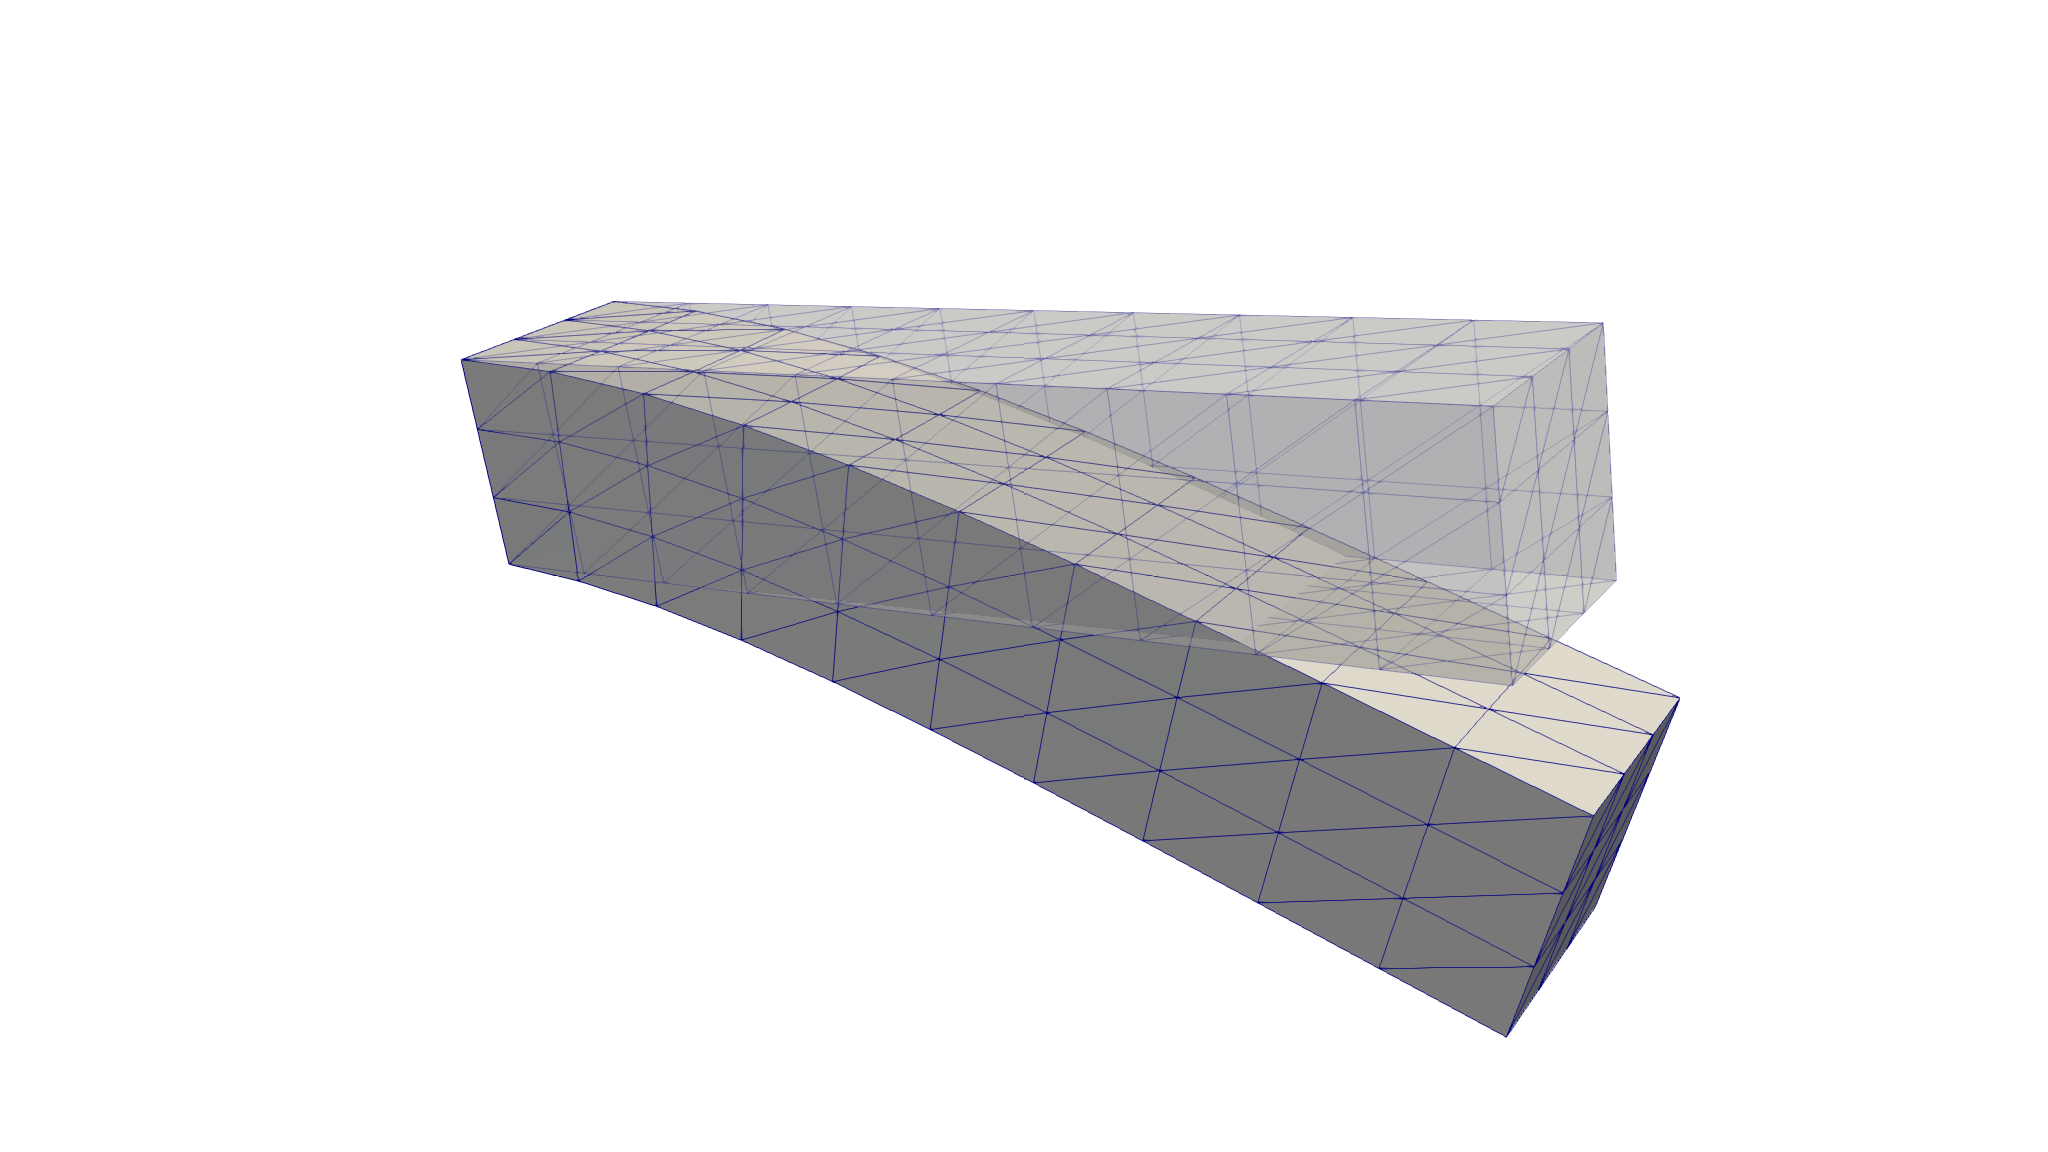
\includegraphics[width=0.45\textwidth]{./images/paper2/beam3d.png} & 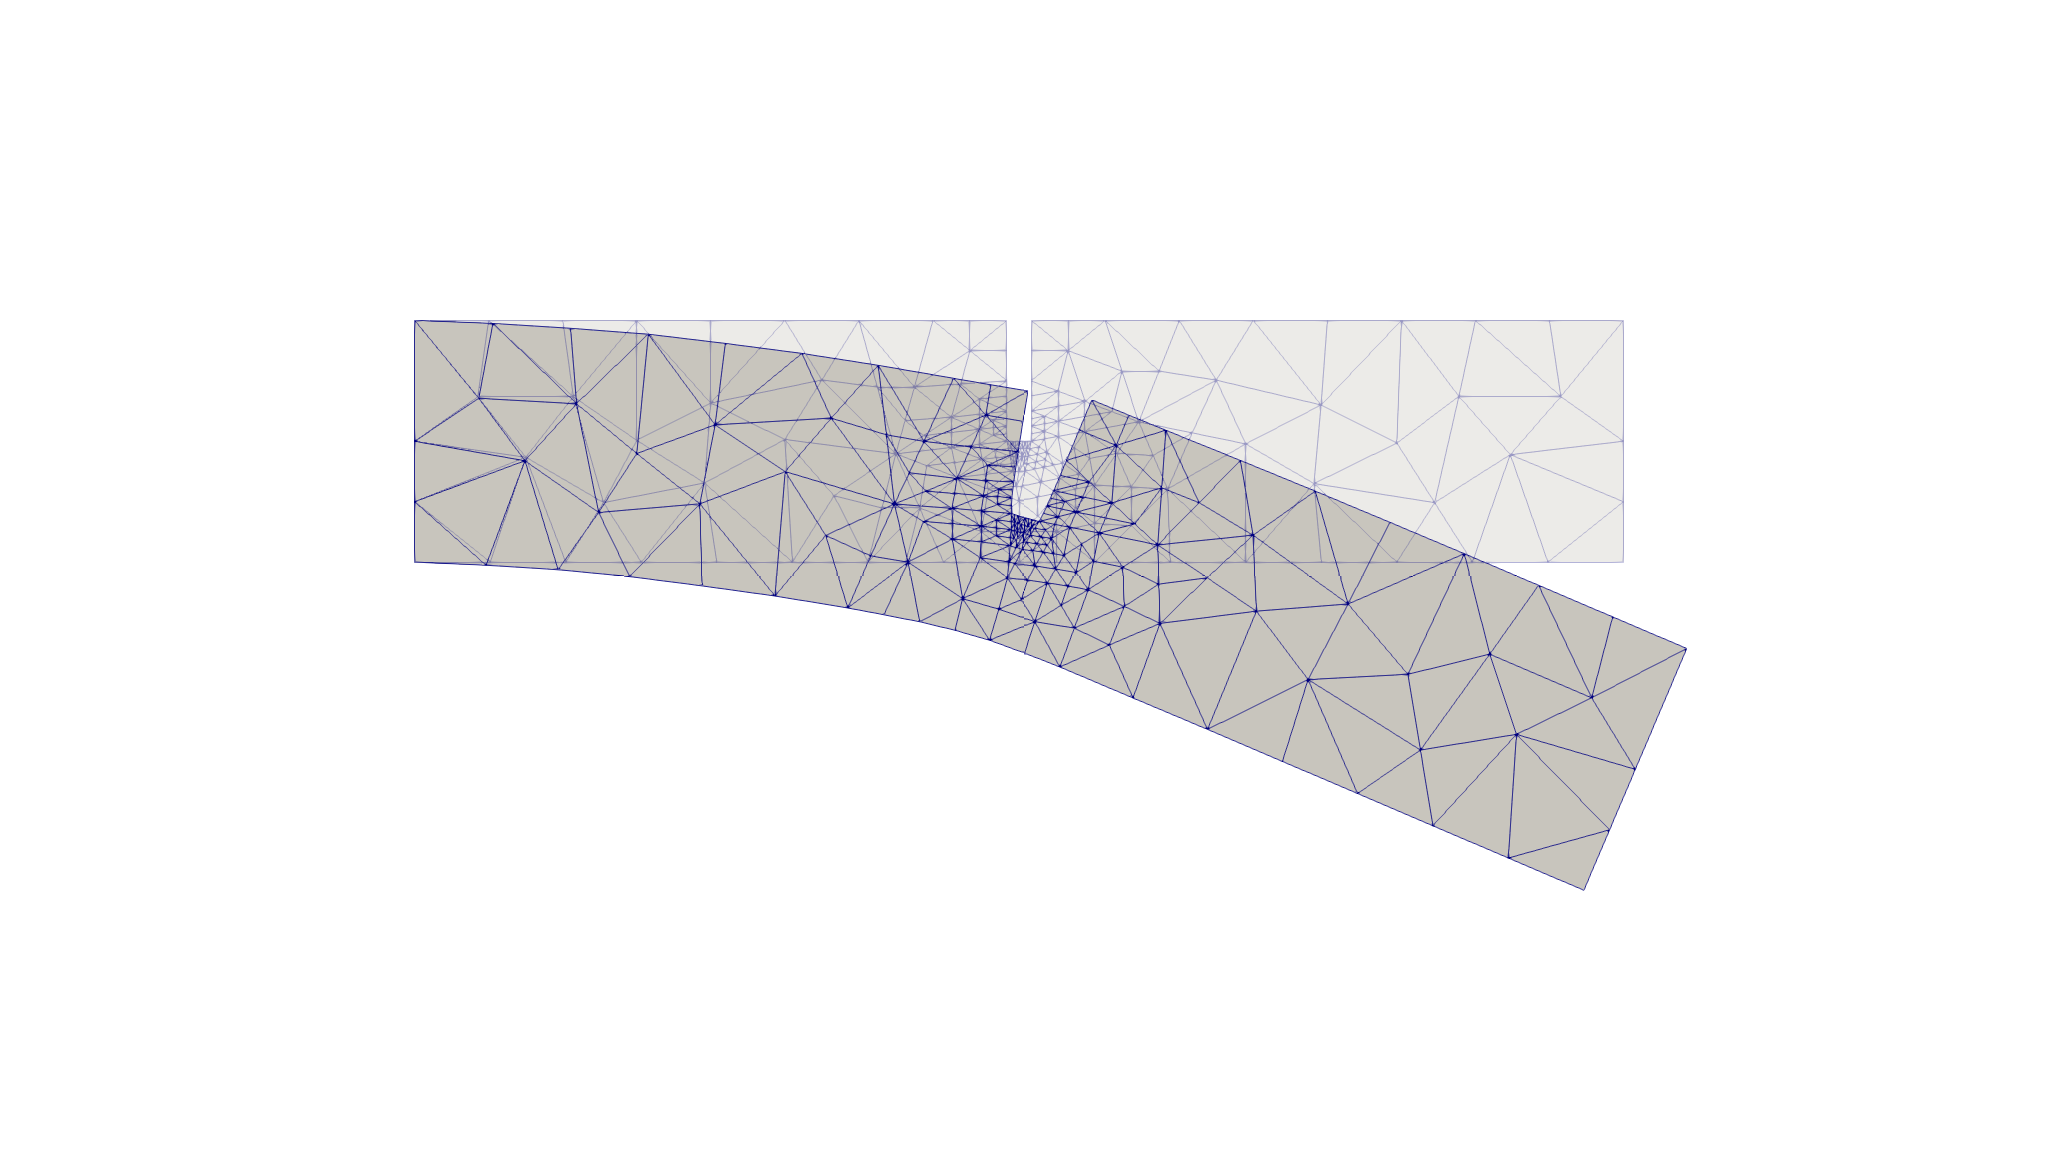
\includegraphics[width=0.45\textwidth]{./images/paper2/beam2d.png} \\
(a) & (b)
\end{tabular}
\caption{(a) initial condition and a snapshot of the 3D beam. (b) initial condition and a snapshot of the 2D beam with a cavity. } \label{fig:0}
\end{figure}

We define a vector valued function space as $V = \{ u \in (L^2(\Gamma))^3 : \| \nabla u_i \|_2 \in L^2 \text{, } i=1,2,3\text{, } u = \vec 0 \text{ on } \partial \Gamma_\tau \}$, equipped with the standard $L^2$ inner product $(\cdot,\cdot):V\times V \to \mathbb R$, and seek the solution to (\ref{eq:res.1}). To derive the weak formulation of (\ref{eq:res.1}), we multiply it with the vector valued test function $v \in V$, integrate over $\Gamma$, and use integration by parts to obtain
%\begin{equation}  \label{eq:res.3}
%	\int_{\Gamma} u_{tt} \cdot v\ dx = \int_{\Gamma} (\nabla \cdot \sigma) \cdot v \ dx + \int_{\Gamma} f \cdot v \ dx.
%\end{equation}
%We may integrate the first term on the right hand side by parts to obtain
\begin{equation}  \label{eq:res.4}
	\int_{\Gamma} u_{tt} \cdot v\ dx = - \int_{\Gamma} \sigma : \nabla v \ dx+ \int_{\partial \Gamma_\tau} (\sigma \cdot n) \cdot v\ ds +  \int_{\Gamma} f \cdot v \ dx,
\end{equation}
where $\sigma : \nabla v = \sum_{i,j}\sigma_{ij}(\nabla v)_{ji}$ is the tensor inner product. Note that the skew-symmetric part of $\nabla v$ vanishes over the product $\sigma : \nabla v$, since $\sigma$ is symmetric. By prescribing the boundary conditions to (\ref{eq:res.4}) we recover
\begin{equation} \label{eq:res.5}
	\int_{\Gamma} u_{tt} \cdot v\ dx = - \int_{\Gamma} \sigma : \text{Sym}(\nabla v) \ dx+ \int_{\partial \Gamma_\tau} \tau \cdot v\ ds +  \int_{\Gamma} f \cdot v \ dx,
\end{equation}
with Sym$(\nabla v) = (\nabla v + (\nabla v)^T)/2$. The variational form associated to (\ref{eq:res.1}) is
\begin{equation} \label{eq:res.6}
	(u_{tt},v) = - a(u,v) + b(v), \quad u,v\in V,
\end{equation}
where
\begin{equation} \label{eq:res.7}
\begin{aligned}
	a(u,v) &= \int_{\Gamma} \sigma : \text{Sym}(\nabla v) \ dx, ~
	b(v) &= \int_{\partial \Gamma_\tau} \tau \cdot v\ ds +  \int_{\Gamma} f \cdot v \ dx.
\end{aligned}
\end{equation}
To obtain the FEM discretization of (\ref{eq:res.6}), we triangulate the domain $\Gamma$ and define vector valued piece-wise linear basis functions $\{\phi_i\}_{i=1}^{N_h}$. We define the FEM space $V_h$, an approximation of $V$, as the span of those basis functions. Projecting (\ref{eq:res.6}) onto $V_h$ yields the discrete weak form
\begin{equation} \label{eq:res.8}
	((u_h)_{tt},v_h) = - a(u_h,v_h) + b(v_h),\quad u_h,v_h\in V_h.
\end{equation}
Any particular function $u_h$ can be expressed as $u_h = \sum_{i=1}^{N_h} q_i \phi_i$, where $q_i$, $i=1,\dots,N_h$, are the expansion coefficients. Therefore, by choosing test functions $v_h = \phi_i$, $i=1,\dots,N_h$, we obtain the system of ODEs
\begin{equation} \label{eq:res.9}
	M\ddot q = -K q + g_{q}.
\end{equation}
where $q=(q_1,\dots,q_{N_h})^T$ are unknowns, the \emph{mass matrix} $M\in \mathbb R^{N_h\times N_h}$ is given as $M_{i,j} = (\phi_i,\phi_j)$, the \emph{stiffness matrix} $K\in \mathbb R^{N_h\times N_h}$ is given as $K_{i,j} = a(\phi_j,\phi_i)$ and $g_q=(b(v_1),\dots,b(v_{N_h}))^T$. Now introduce the canonical coordinate $p = M\dot q$ to recover the Hamiltonian system
\begin{equation} \label{eq:res.10}
	\dot z = \mathbb J_{2N_h} Lz + g_{qp},
\end{equation}
where
\begin{equation} \label{eq:res.11}
	z = 
	\begin{pmatrix}
	q \\
	p	
	\end{pmatrix}, \quad 
	L = 
	\begin{pmatrix}
	K & 0 \\
	0 & M^{-1}
	\end{pmatrix}, \quad
	g_{qp} =
	\begin{pmatrix}
	0 \\
	g_q
	\end{pmatrix},
\end{equation}
together with the Hamiltonian function $H(z) = \frac{1}{2} z^TLz + z^T \mathbb J_{2N_h}^T g_{qp}$. An appropriate FEM setup leads to a symmetric and positive-definite matrix $L$. Hence, it seems natural to take $X=L$, the energy matrix associated to (\ref{eq:res.10}). The system parameters are summarized in the table below. For further information regarding the problem, we refer to \cite{langtangen2017solving}.

\vspace{0.5cm}
\begin{center}
\begin{tabular}{|l|l|}
\hline
Domain shape & box: $l_x = 1,\ l_y = 0.2,\ l_z = 0.2$ \\
Time step-size & $\Delta t = 0.01$ \\
Gravitational force & $f = (0,0,-0.4)^T$ \\
Traction & $\tau = \vec 0$ \\
Lam\'e parameters & $\lambda = 1.25$, $\mu = 1.0$ \\
Degrees of freedom & $2N_{h} = 1650$ \\
\hline
\end{tabular}
\end{center}
\vspace{0.5cm}
Projection operators $P_{X,V}$, $P^{\text{symp}}_{I,A}$ and $P^{\text{symp}}_{X,\tilde A}$ are constructed following \Cref{alg:3.2,alg:4.1,alg:5.1}, respectively, with $\delta = 5\times 10^{-4}, 2\times 10^{-4}$ and $1\times 10^{-4}$. The reduced systems, obtained from $P^{\text{symp}}_{I,A}$ and $P^{\text{symp}}_{X,\tilde A}$, are integrated in time using the St\"ormer-Verlet scheme to generate the temporal snapshots. The reduced system obtained from $P_{X,V}$ is integrated using a second order implicit Runge-Kutta method. Note that the St\"ormer-Verlet scheme is not used since the canonical form of a Hamiltonian system is destroyed when $P_{X,V}$ is applied.

\begin{figure}[t] 
\begin{tabular}{cc}
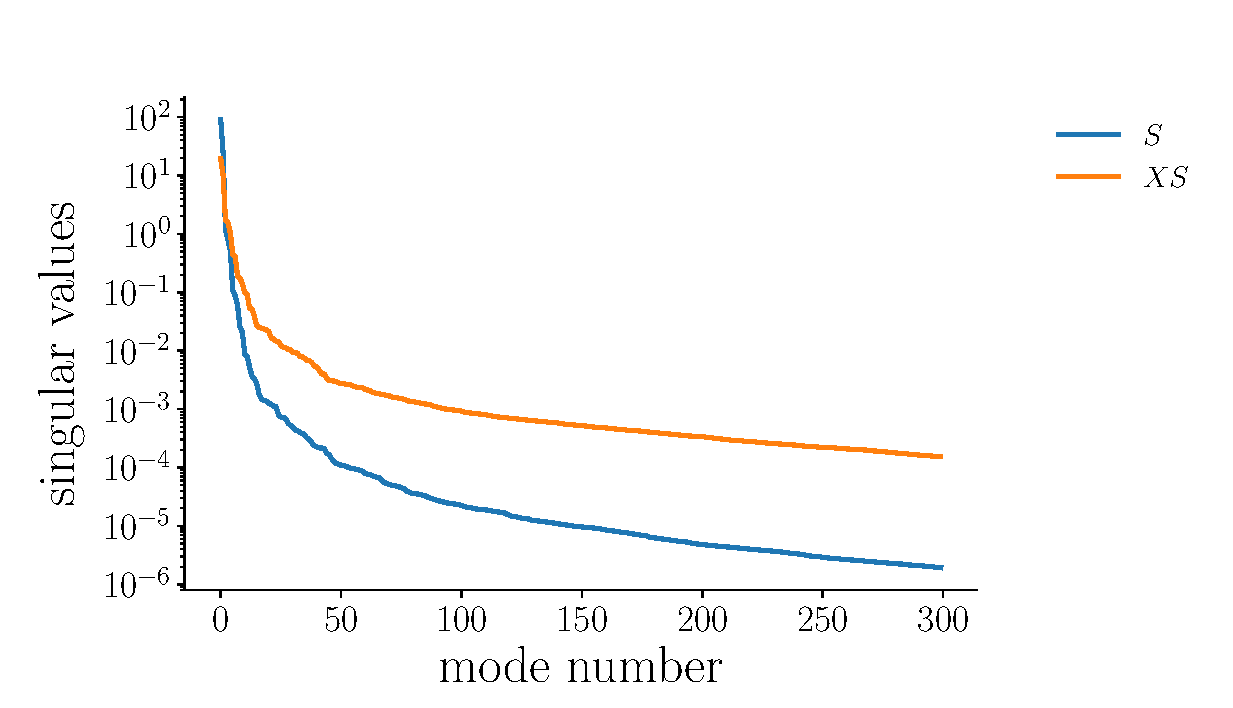
\includegraphics[width=0.45\textwidth]{./images/paper2/beam/singulars} & 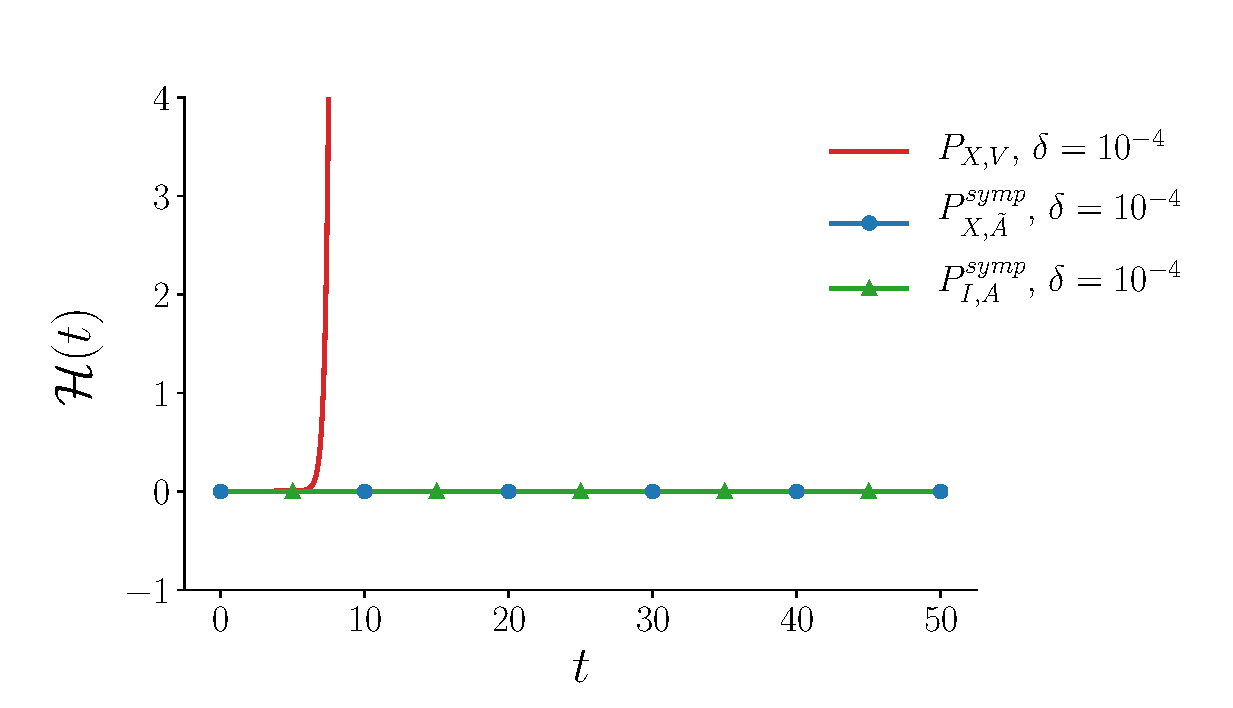
\includegraphics[width=0.45\textwidth]{./images/paper2/beam/energy} \\
(a) & (b) \\
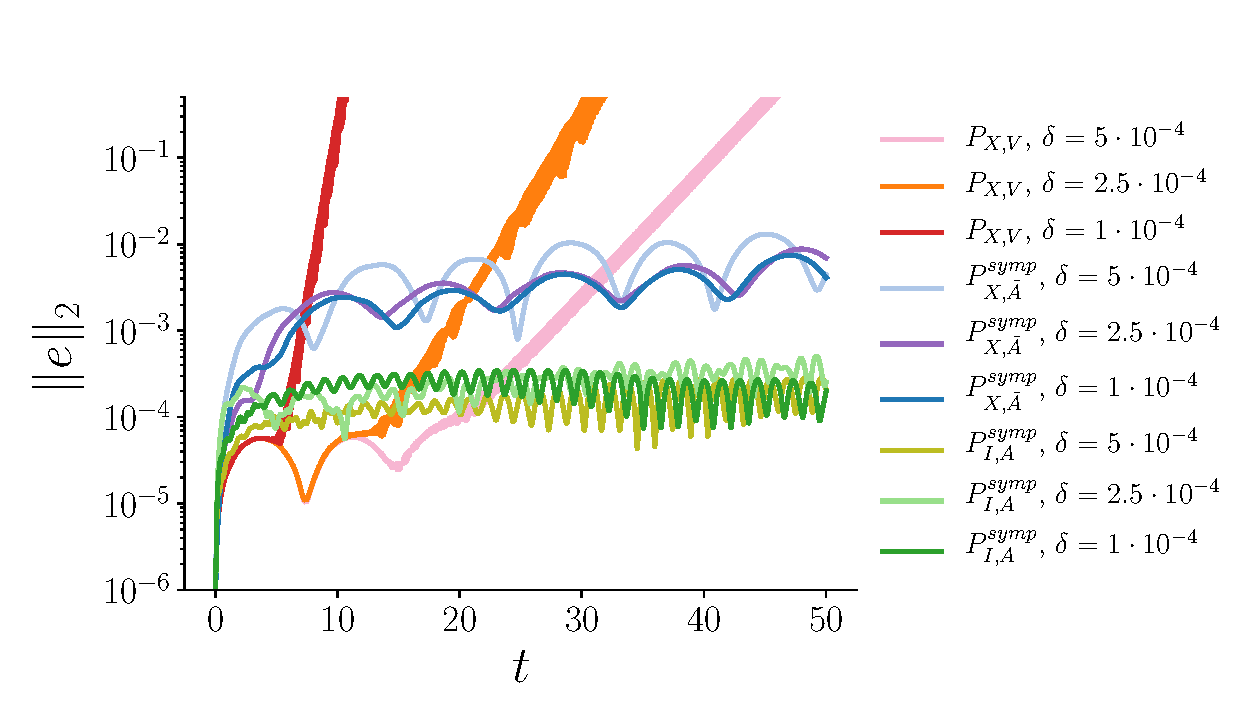
\includegraphics[width=0.45\textwidth]{./images/paper2/beam/l2_norm} & 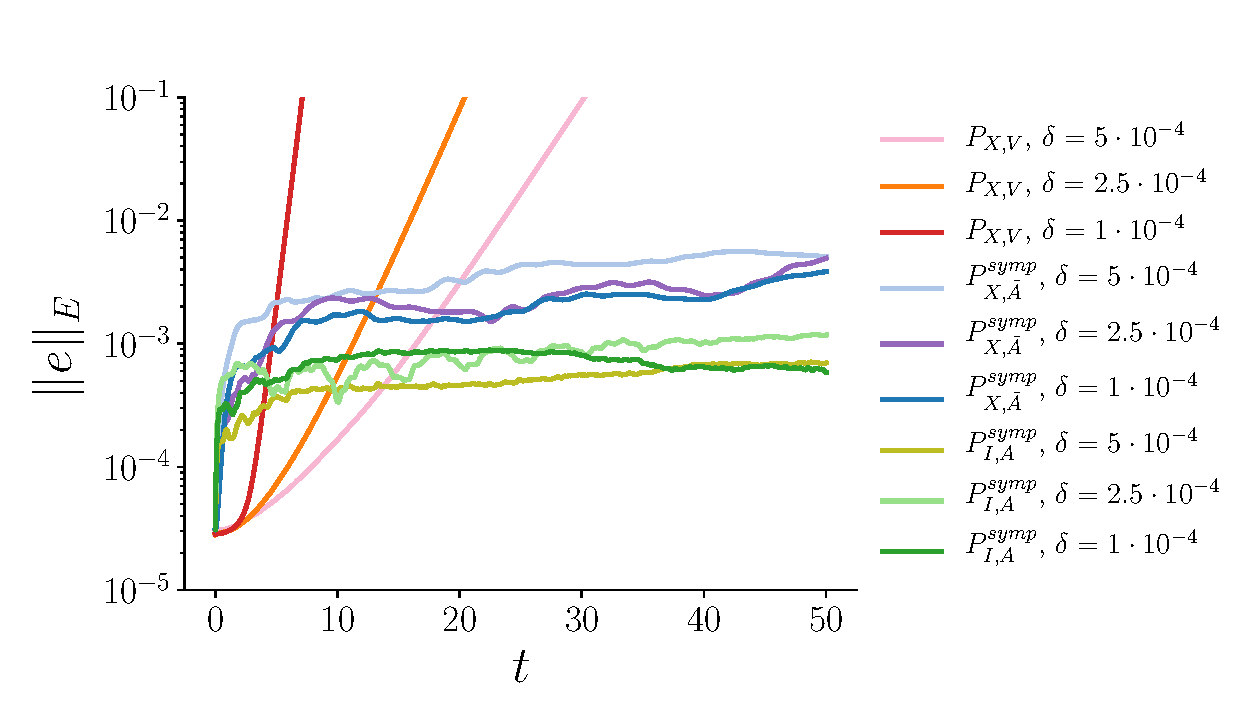
\includegraphics[width=0.45\textwidth]{./images/paper2/beam/energy_norm} \\
(c) & (d) \\
\end{tabular}
\caption{Numerical results related to the beam equation. (a) the decay of the singular values, (b) conservation of the Hamiltonian, (c) error with respect to the 2-norm, (d) error with respect to the $X$-norm.} \label{fig:1}
\end{figure}

\Cref{fig:1}.(a) shows the decay of the singular values of the temporal snapshots $S$ and $XS$, respectively. The difference in the decay indicates that the reduced systems constructed using $P_{I,A}^{\text{symp}}$ and $P_{X,\tilde A}^{\text{symp}}$ would have different sizes for a similar prescribed accuracy.

\Cref{fig:1}.(b) shows the conservation of the Hamiltonian for the methods discussed previously. This confirms that the symplectic methods preserve the Hamiltonian and the system energy. However, the Hamiltonian blows up for the reduced system constructed by the projection $P_{X,V}$.

\Cref{fig:1}.(c) shows the $L^2$ error between the projected systems and the full order system, defined as
\begin{equation}
	\| e \|_{L^2} = \sqrt{(e,e)} \approx \sqrt{ (q - \hat q)^T M (q-\hat q) },
\end{equation}
where $e\in V$ is the error function and $\hat q \in \mathbb R^{2n}$ is an approximation for $q$. We notice that the reduced system obtained by the non-symplectic method is unstable and the reduced system, constructed using $P_{X,V}$, is more unstable as $k$ increases. On the other hand, the symplectic methods yield a stable reduced system. Although the system, constructed by the projection $P^{\text{symp}}_{X,\tilde A}$, is not based on the 2-norm projection, the error remains bounded with respect to the 2-norm. 

We define the energy norm $\| \cdot \|_E : V \to \mathbb R$ as
\begin{equation}
	\| (u,\dot u) \|_E = \sqrt{ a(u,u) + (\dot u , \dot u) } \approx \| z \|_X.
\end{equation}
\Cref{fig:1}.(d) shows the MOR error with respect to the energy norm. We observe that the classical model reduction method based on the projection $P_{X,V}$ does not yield a stable reduced system. However, the symplectic methods provide a stable reduced system. We observe that the original symplectic approach also provides an accurate solution with respect to the energy norm. Nevertheless, the relation between the two norms depends on the problem set up and the choice of discretization \cite{DEPARIS20094359}.

\subsection{Elastic Beam With Cavity}  \label{sec:res.1.1}
In this section we investigate the performance of the proposed method on a two dimensional elastic beam that contains a cavity. In this case a nonuniform triangulated mesh is desirable to balance the computational cost of a FEM discretization with the numerical error around the cavity. \Cref{fig:0}.(a) shows the nonuniform mesh used in this section.
System parameters are taken to be identical to those in \Cref{sec:res.1}. Numerical parameters are summarized in the table below.
\vspace{0.5cm}
\begin{center}
\begin{tabular}{|l|l|}
\hline
cavity width & $l_c = 0.1$ \\
Time step-size & $\Delta t = 4\times 10^{-4}$ \\
Degrees of freedom & $2N_{h} = 744$ \\
\hline
\end{tabular}
\end{center}
\vspace{0.5cm}


\begin{figure} 
\begin{tabular}{cc}
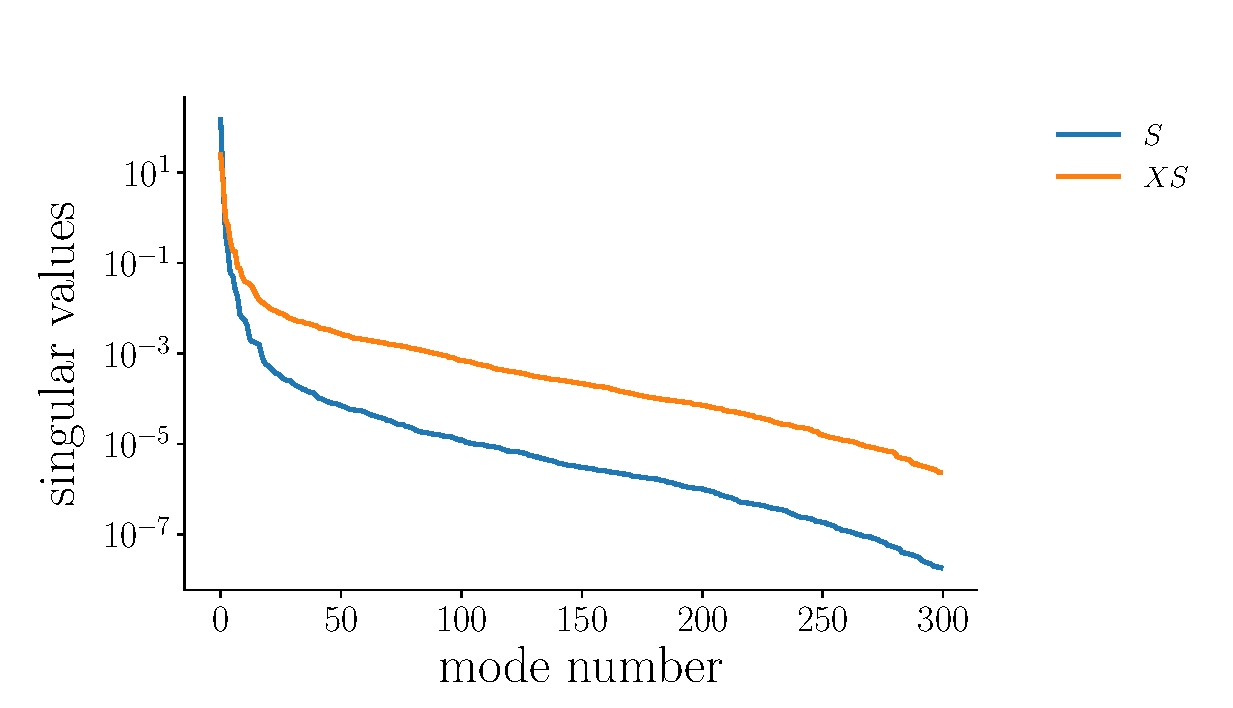
\includegraphics[width=0.45\textwidth]{./images/paper2/beam_cracked/singulars} & 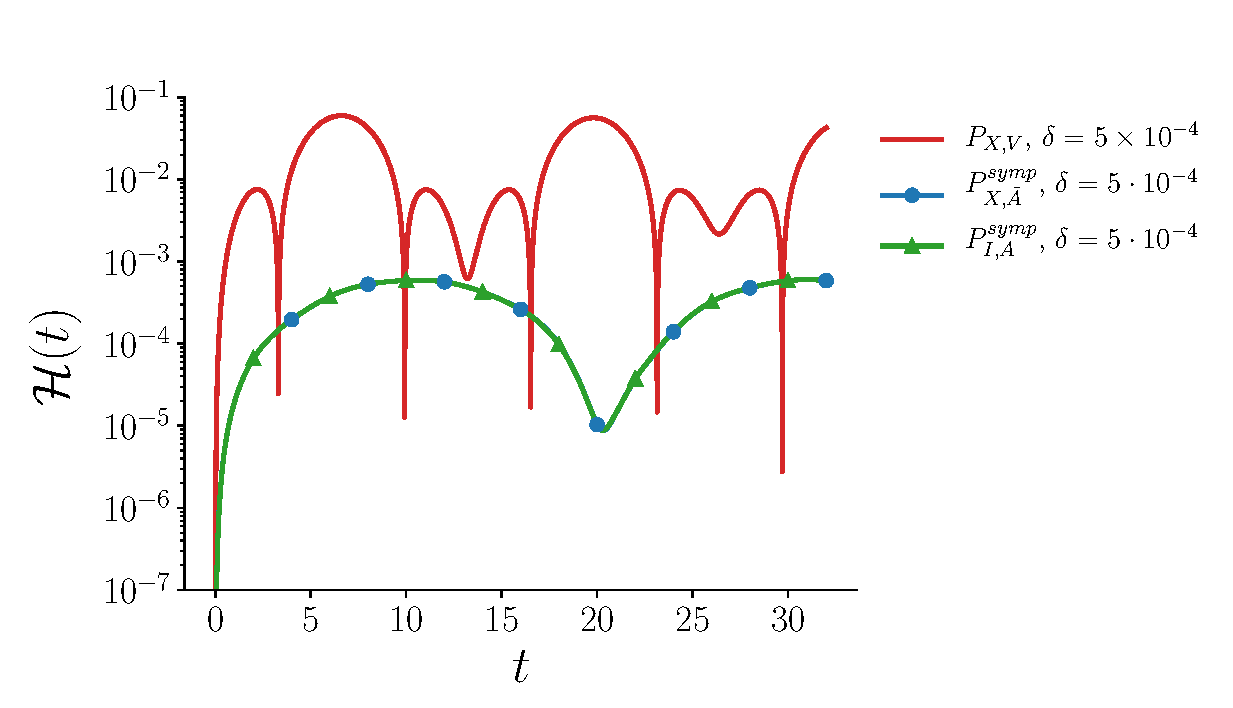
\includegraphics[width=0.45\textwidth]{./images/paper2/beam_cracked/energy} \\
(a) & (b) \\
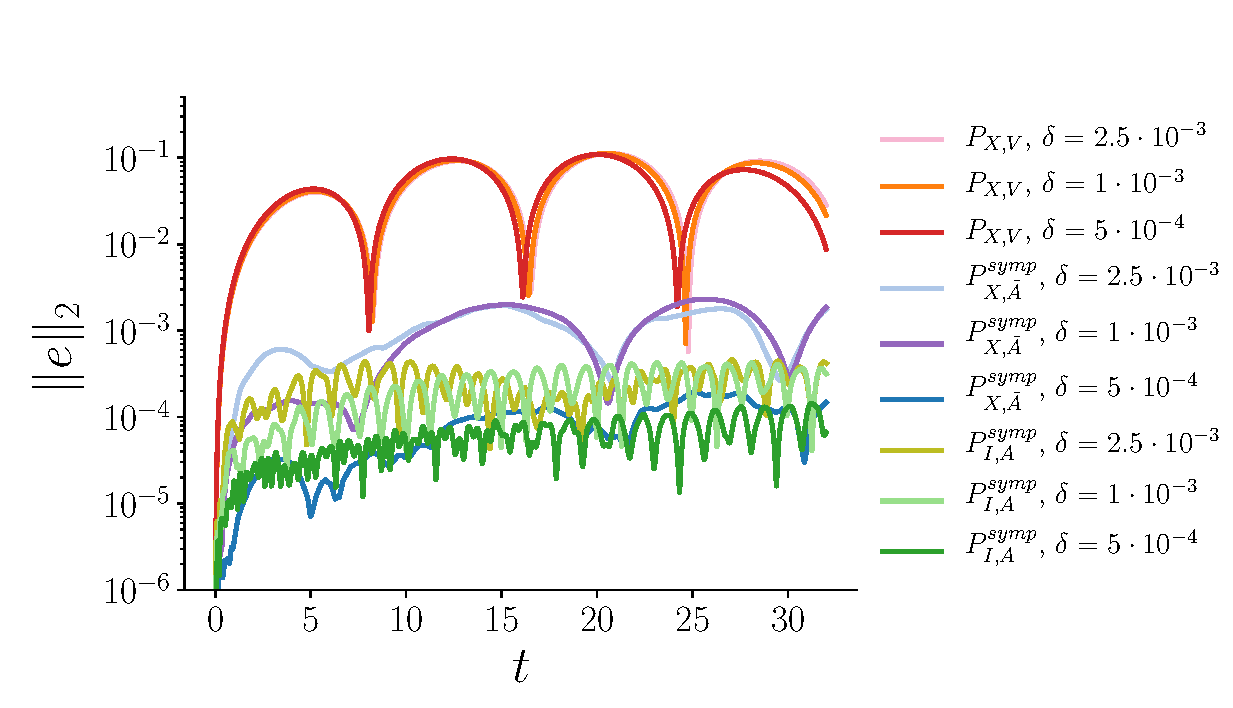
\includegraphics[width=0.45\textwidth]{./images/paper2/beam_cracked/l2} & 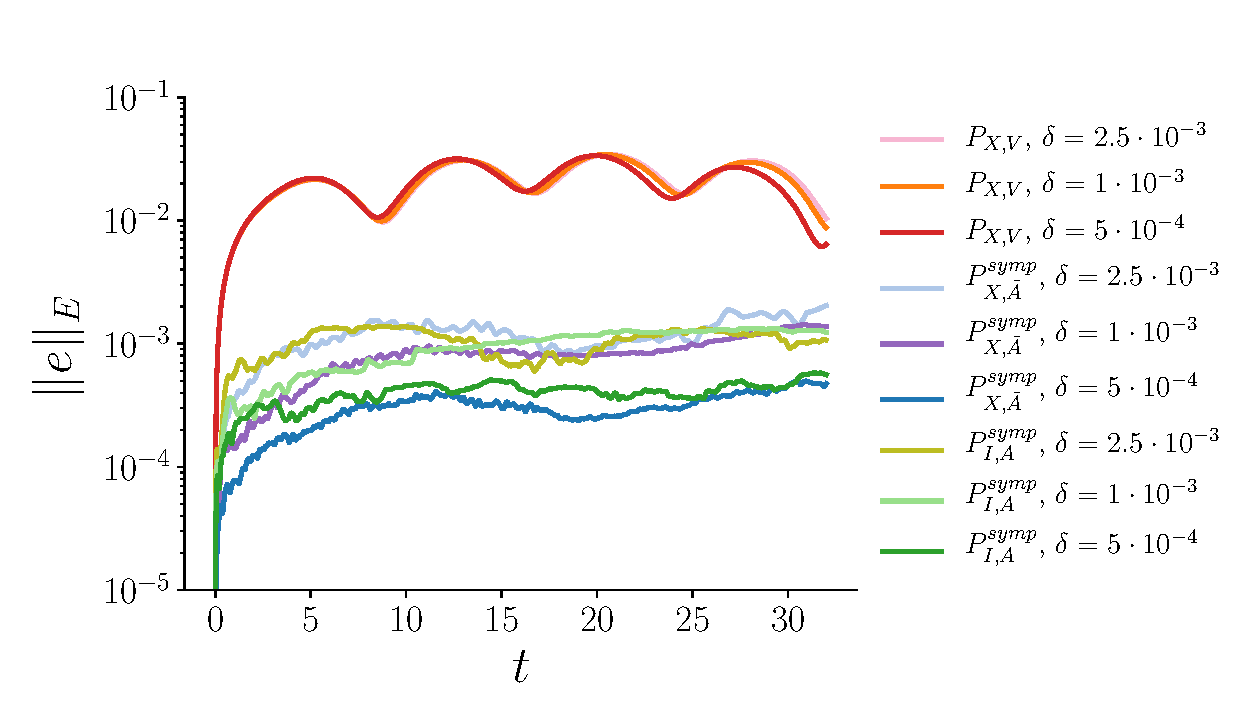
\includegraphics[width=0.45\textwidth]{./images/paper2/beam_cracked/energy_norm} \\
(c) & (d) \\
\end{tabular}
\caption{Numerical results related to the beam with cavity. (a) the decay of the singular values, (b) conservation of the Hamiltonian, (c) error with respect to the 2-norm, (d) error with respect to the energy norm.} \label{fig:1.1}
\end{figure}

\Cref{fig:1.1}.(a) shows the decay of the singular values for the snapshot matrix $S$ and $XS$. The divergence of the two curves indicates that to obtain the same accuracy in the reduced system, the basis constructed from $S$ and $XS$ would have different sizes.
Projection operators $P_{X,A}$, $P_{I,A}^{\text{symp}}$ and $P_{X,\tilde A}^{\text{symp}}$ are constructed according to the \Cref{alg:3.2,alg:4.1,alg:5.1}. The error tolerated is set to $\delta = 2.5\times 10^{-3}$, 
$\delta = 1\times 10^{-3}$ and $\delta = 5\times 10^{-4}$.

The 2-norm error and the error in the energy norm are presented in \Cref{fig:1.1}.(c) and \Cref{fig:1.1}.(d), respectively. We notice that although the non-symplectic method is bounded, it results in larger errors compared to the symplectic methods. Moreover, we notice that the error generated by the symplectic methods is consistently reduced under basis enrichment. It is observed that in the energy norm, the projection $P_{X,\tilde A}^{\text{symp}}$ provides a more accurate solution by comparing to \Cref{fig:1}. This is due to the nonuniform mesh on which the weight matrix $X$ associates higher weights to the elements that are subject to larger error. Therefore, we expect the reduced system constructed with the projection $P_{X,\tilde A}^{\text{symp}}$, to outperform the one constructed with $P_{I,A}^{\text{symp}}$ on a highly nonuniform mesh.

\Cref{fig:1.1}.(b) shows the error in the Hamiltonian. Comparing to \Cref{fig:1}, we notice that the energy norm strengthens the boundedness of the non-symplectic method. However, the symplectic methods preserves the Hamiltonian at a higher accuracy

\subsection{The sine-Gordon equation} \label{sec:res.2}
The sine-Gordon equation arises in differential geometry and quantum physics \cite{Misumi2015}, as a nonlinear generalization of the linear wave equation of the form
\begin{equation} \label{eq:res.12}
\left\{
\begin{aligned}
	u_{t}(t,x) &= v, \quad x\in \Gamma,\\
	v_t(t,x) &= u_{xx} - \sin(u), \\
	u(t,0) &= 0, \\
	u(t,l) &= 2\pi.
\end{aligned}
\right.
\end{equation}
Here $\Gamma = [0,l]$ is a line segment and $u,v: \Gamma \to \mathbb R$ are scalar functions. The Hamiltonian associated with (\ref{eq:res.12}) is
\begin{equation} \label{eq:res.13}
	H(q,p) = \int_{\Gamma} \frac 1 2 v^2 + \frac 1 2 u_x^2 + 1 - \cos(u) \ dx.
\end{equation}
One can verify that $u_{t} = \delta_v H$ and $v_{t} = - \delta_u H$, where $\delta_v,\delta_u$ are standard variational derivatives. The sine-Gordon equation admits the soliton solution \cite{Misumi2015}
\begin{equation} \label{eq:res.14}
	u(t,x) = 4 \text{arctan}\left( \exp \left( \pm \frac{x - x_0 - ct}{\sqrt{1-c^2}} \right) \right),
\end{equation}
where $x_0 \in \Gamma$ and the plus and minus signs correspond to the \emph{kink} and the \emph{anti-kink} solutions, respectively. Here $c$, $|c|<1$, is the wave speed. We discretize the segment into $n$ equi-distant grid point $x_i = i\Delta x$, $i=1,\dots,n$. Furthermore, we use a standard finite-differences scheme to discretize (\ref{eq:res.12}) and obtain
\begin{equation} \label{eq:res.15}
	\dot z = \mathbb J_{2n} L z + \mathbb J_{2n} g(z) + \mathbb J_{2n} c_b.
\end{equation}
Here $z = (q^T,p^T)^T$, $q(t) = (u(t,x_1),\dots,u(t,x_N))^T$, $p(t) = (v(t,x_1),\dots,v(t,x_N))^T$, $c_b$ is the term corresponding to the boundary conditions and
\begin{equation} \label{eq:res.16}
	L = 
	\begin{pmatrix}
		D_x^TD_x & 0_N \\
		0_N & I_n
	\end{pmatrix}, 
	\quad
	g(z) = 
	\begin{pmatrix}
	\sin(q) \\
	\vec 0
	\end{pmatrix},
\end{equation}
where $D_x$ is the standard matrix differentiation operator. We may take $X = L$ as the weight matrix associated to (\ref{eq:res.15}). The discrete Hamiltonian takes the form
\begin{equation} \label{eq:res.17}
	H_{\Delta x} = \Delta x \cdot \frac 1 2 \| p \|^2_2 + \Delta x \cdot \| D_x q \|^2_2 + \sum_{i=1}^{n} \Delta x \cdot ( 1 - \cos(q_i) ).
\end{equation}
The system parameters are given as
\vspace{0.5cm}
\begin{center}
\begin{tabular}{|l|l|}
\hline
Domain length & $l = 50$ \\
No. grid points & $n = 500$ \\
Time step-size & $\Delta t = 0.01$ \\
Wave speed & $c=0.2$ \\
\hline
\end{tabular}
\end{center}
\vspace{0.5cm}
The midpoint scheme \eqref{eq:2.25} is used to integrate (\ref{eq:res.12}) in time and generate the snapshot matrix $S$. Similar to the previous subsection, projection operators $P_{X,V}$, $P^{\text{symp}}_{I,A}$ and $P^{\text{symp}}_{X,\tilde A}$ are used to construct a reduced system. To accelerate the evaluation of the nonlinear term, the symplectic DEIM and the generalized symplectic DEIM, \Cref{alg:5.2}, are coupled with the projection operators $P^{\text{symp}}_{I,A}$ and $P^{\text{symp}}_{X,A}$, respectively. Furthermore, the DEIM approximation is used for the efficient evaluation of the reduced system, obtained by the projection $P_{X,V}$. The midpoint rule is also used to integrate the reduced systems in time. \Cref{fig:2} shows the numerical results obtained with the reduced models without approximating the nonlinearity, while the results for the accelerated evaluation of the nonlinear term are presented in \Cref{fig:3}.

\begin{figure} 
\begin{tabular}{cc}
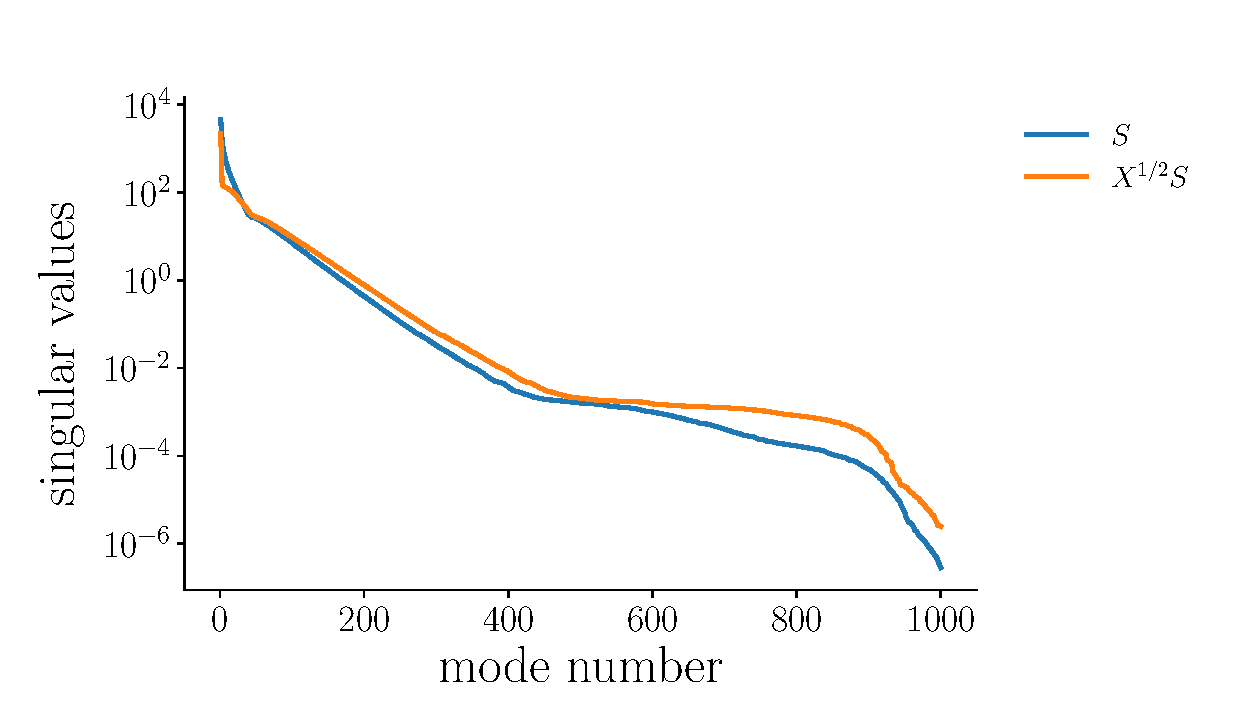
\includegraphics[width=0.45\textwidth]{./images/paper2/sine/singulars} & 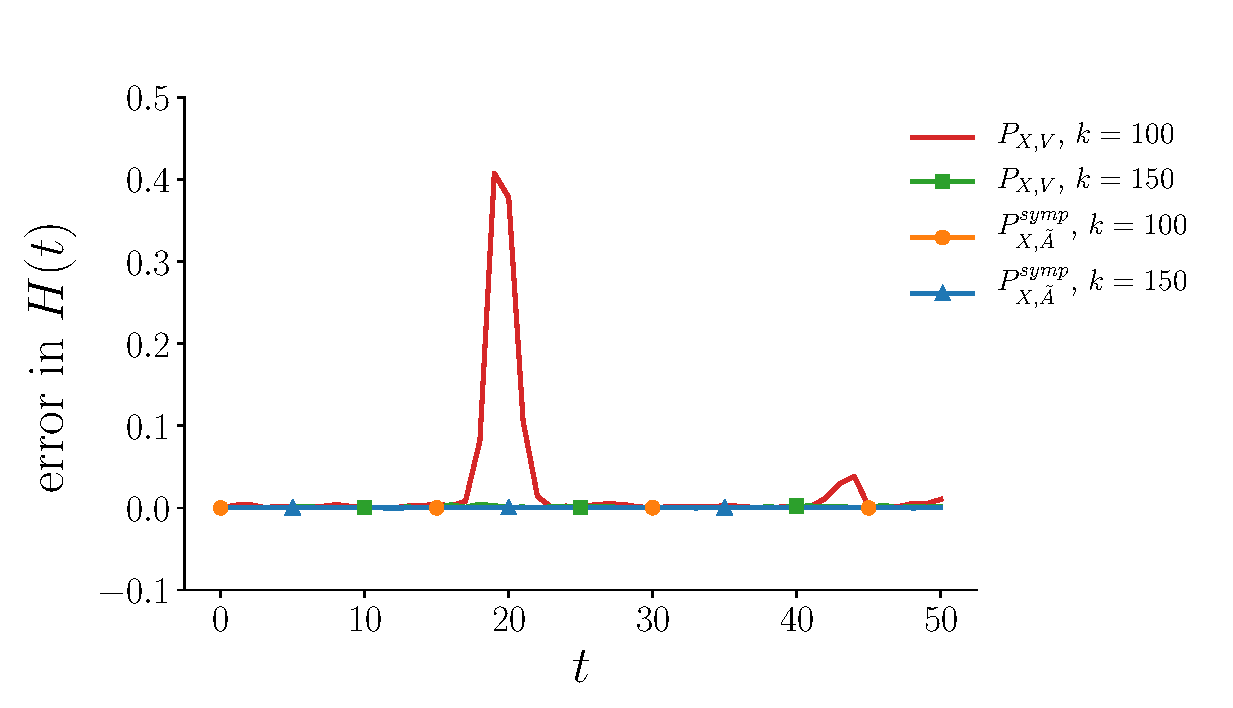
\includegraphics[width=0.45\textwidth]{./images/paper2/sine/energy} \\
(a) & (b) \\
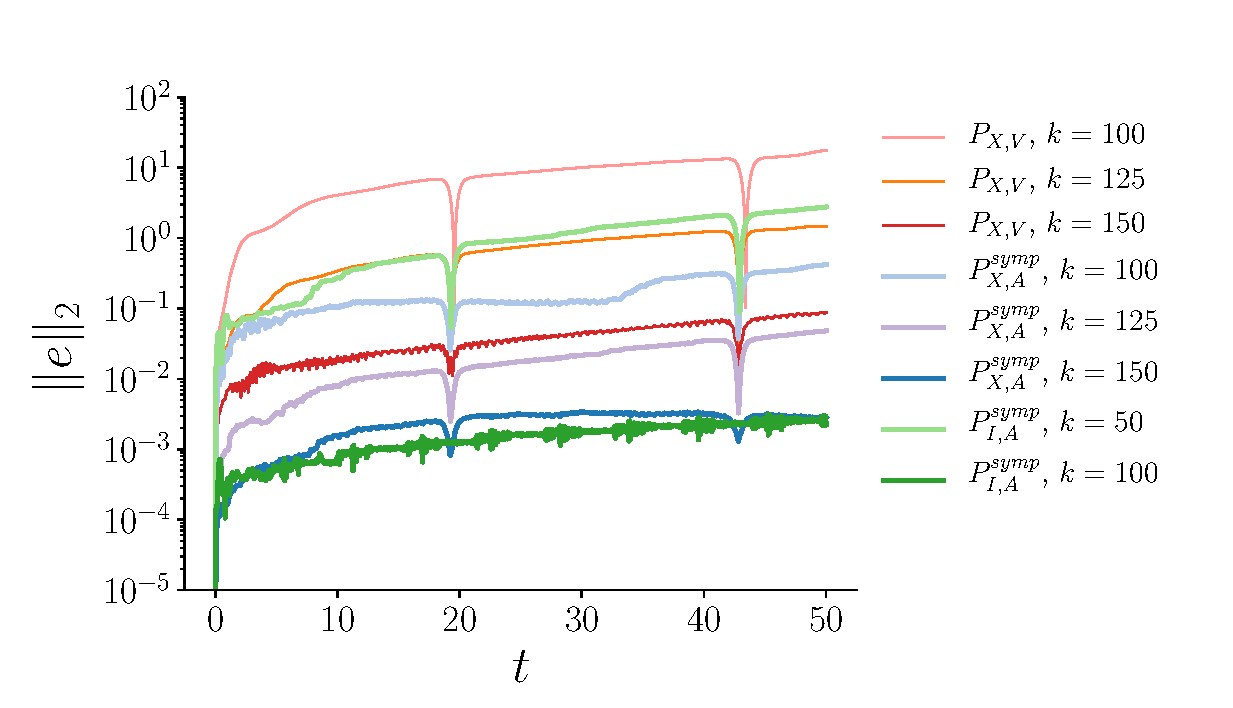
\includegraphics[width=0.45\textwidth]{./images/paper2/sine/l2} & 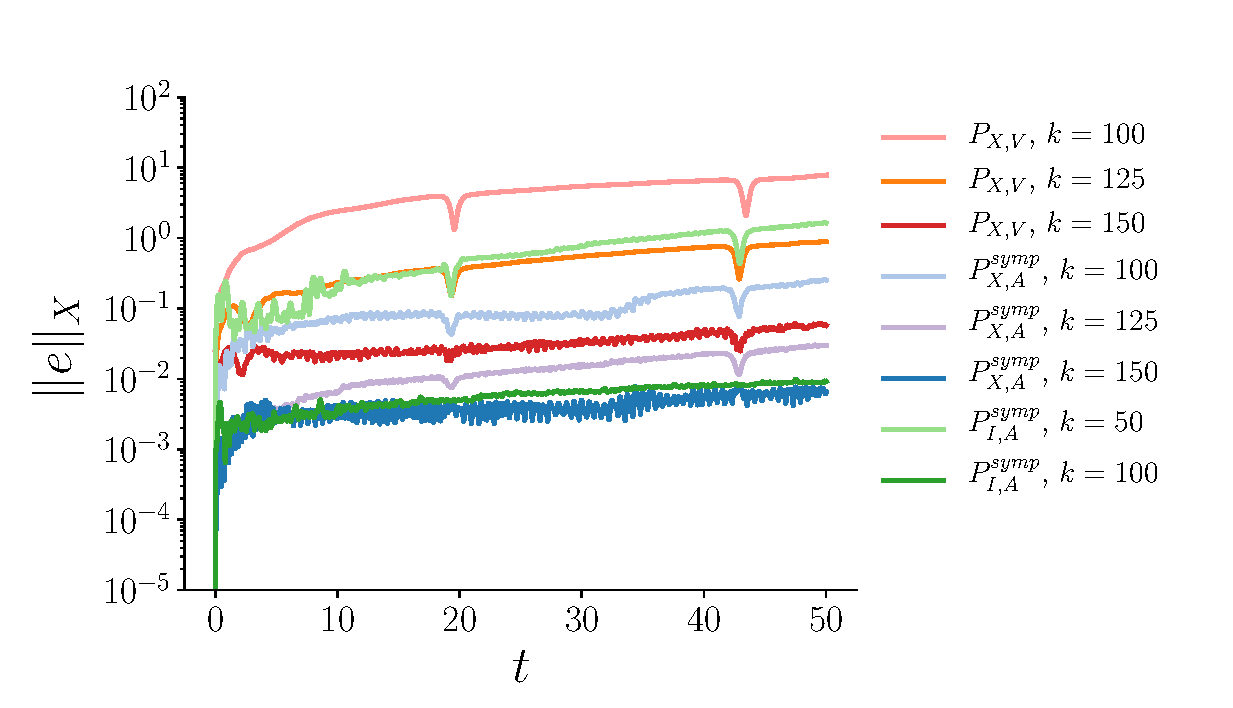
\includegraphics[width=0.45\textwidth]{./images/paper2/sine/energy_norm} \\
(c) & (d) \\
\end{tabular}
\caption{Numerical results related to the sine-Gordon equation. (a) the decay of the singular values, (b) the error in the Hamiltonian, (c) the error with respect to the 2-norm, (d) the error with respect to the energy norm.} \label{fig:2}
\end{figure}

\Cref{fig:2}.(a) shows the decay of the singular values of matrices $S$ and $XS$. As previously, we observe a saturation in the decay of the singular values of $XS$ compared to the singular values of $S$. This indicates that the reduced basis, based on a weighted inner product, should be chosen to be larger to provide an accuracy similar to based on the Euclidean inner product. Put differently, unweighted reduced bases, when compared to the weighted ones, may be highly inaccurate in reproducing the underlying physical properties of the system.

\Cref{fig:2}.(b) displays the error in the Hamiltonian. It is again observed that the symplectic approaches conserve the Hamiltonian. However, the classic approaches do not necessarily conserve the Hamiltonian. We point out that using the projection operator $P_{X,V}$ ensures the boundedness of the Hamiltonian. The contrary is observed when we apply the POD with respect to the Euclidean inner-product, i.e. applying the projection operator $P_{I,V}$. This can be seen in the results presented in \cite{doi:10.1137/140978922}, where the unboundedness of the Hamiltonian is observed when $P_{I,V}$ is applied to the sine-Gordon equation. Nevertheless, only the symplectic model reduction consistently preserves the Hamiltonian.

\Cref{fig:2}.(c) shows the error with respect to the Euclidean inner-product between the solution of the projected systems and the original system. The behavior of the solution is investigated for $k=100$, $k=125$ and $k=150$. We observe that all systems that are projected with respect to the $X$-norm are bounded. As the results in \cite{doi:10.1137/140978922} suggest, the Euclidean inner-product does not necessarily yield a bounded reduced system. Moreover, we notice that the symplectic projection $P^{\text{symp}}_{X,\tilde A}$ results in a substantially more accurate reduced system compared to the reduced system yielded from $P_{X,V}$. This is because the overall behavior of the original system is translated correctly to the reduced system through the symplectic projection.

The error with respect to the $X$-norm between the solution of the original system and the projected systems is presented in \Cref{fig:2}.(d). We observe that the behavior of the $X$-norm error is similar to that in the Euclidean norm. However, the growth of the error is slower for methods based on a weighted inner product. Note that the connection between the error in the Euclidean norm and the $X$-norm is problem and discretization dependent. We also observe that symplectic methods are substantially more accurate.

\begin{figure} 
\begin{tabular}{cc}
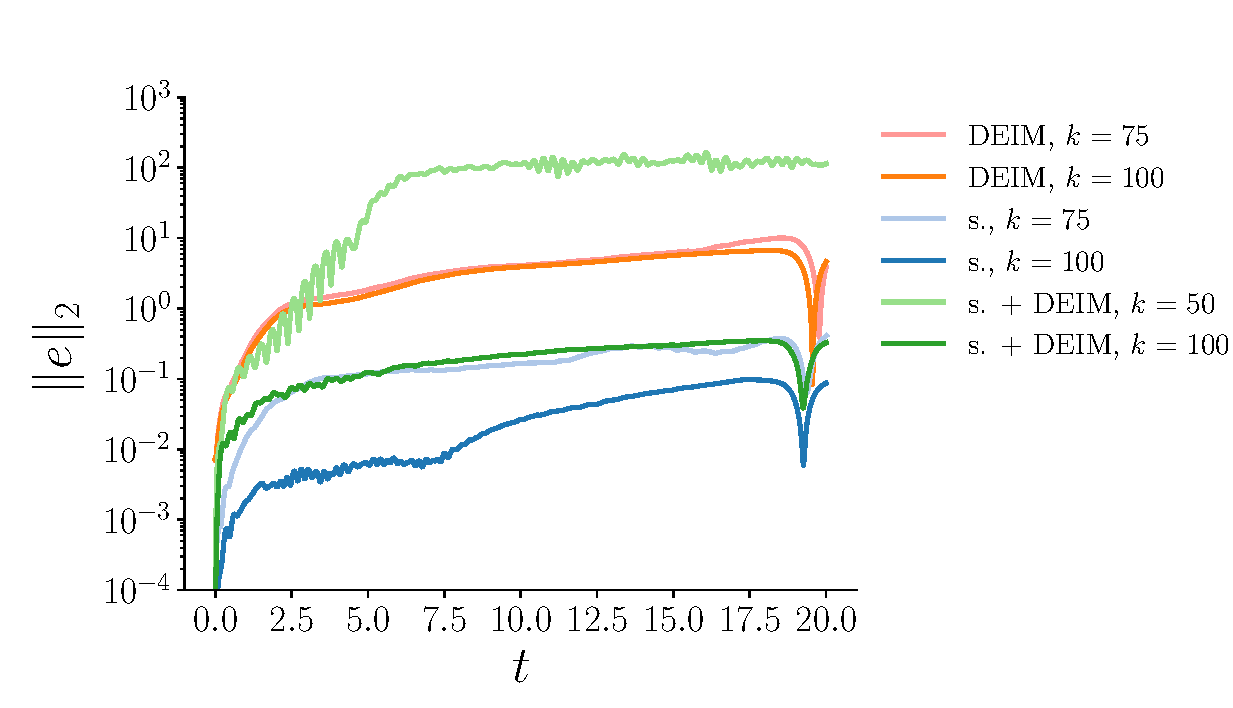
\includegraphics[width=0.45\textwidth]{./images/paper2/sine/nonlinear/l2} & 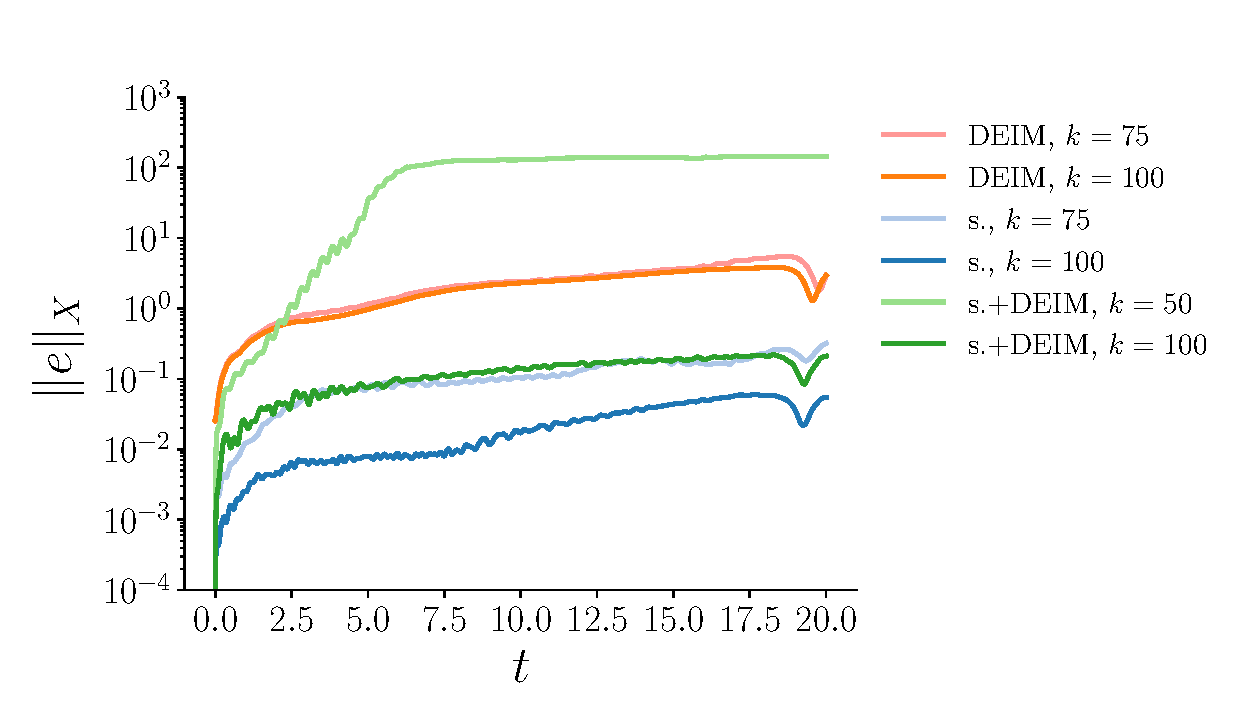
\includegraphics[width=0.45\textwidth]{./images/paper2/sine/nonlinear/energy_norm} \\
(a) & (b) \\
\multicolumn{2}{c}{
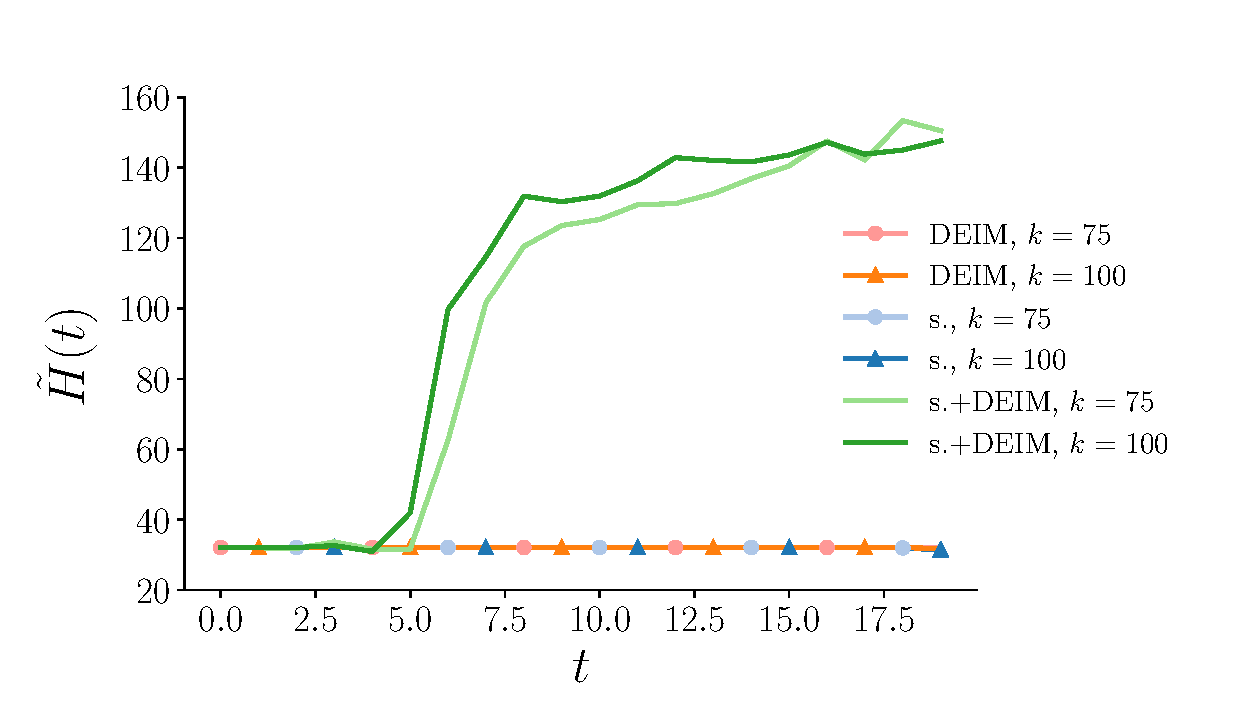
\includegraphics[width=0.45\textwidth]{./images/paper2/sine/nonlinear/energy}
} \\
\multicolumn{2}{c}{(c)} \\
\end{tabular}
\caption{Numerical results related to the sine-Gordon equation with efficient evaluation of the nonlinear terms. Here, ``DEIM'' indicates classical model reduction with the DEIM, ``s.+DEIM'' indicates symplectic model reduction with the DEIM and ``s.'' indicates symplectic model reduction with symplectic treatment of the nonlinear term. (a) error with respect to the Euclidean norm, (b) error with respect to the $X$-norm, (c) error in the Hamiltonian. } \label{fig:3}
\end{figure}

\Cref{fig:3} shows the performance of the different model reduction methods, when an efficient method is adopted for evaluating the nonlinear term in (\ref{eq:res.15}). This figure compares the symplectic approaches against non-symplectic methods. For all simulations, the size of the reduced basis for (\ref{eq:res.15}) is chosen to be $k=100$. The size of the basis of the nonlinear term is taken as $k_n=75$ and $k_n=100$. For symplectic methods, a basis for the nonlinear term is constructed according to \Cref{alg:5.2}, whereas for non-symplectic methods, the DEIM is applied. Note that for symplectic methods, the basis for the nonlinear term is added to the symplectic basis $A$. This means that the size of the reduced system is larger when compared to the classical approach.

\section{Conclusion} \label{sec:conc}
This chapter presents a model reduction approach that combines the classic model reduction method, defined with respect to a weighted inner product, with symplectic model reduction. This allows the reduced system to be defined with respect to norms and inner-products that are natural to the problem and most suitable for the method of discretization. Furthermore, the symplectic nature of the reduced system preserves the Hamiltonian structure of the original system, which results in robustness and enhanced stability in the reduced system.

It is demonstrated that including the weighted inner-product in the symplectic model reduction can be viewed as a natural extension of the unweighted symplectic method. Therefore, the stability preserving properties of the symplectic method generalize naturally to the new method.

Numerical results suggest that classic model reduction methods with respect to a weighted inner product can help with the boundedness of the system. However, only the symplectic treatment can consistently increase the accuracy of the reduced system. This is consistent with the fact the symplectic methods preserve the Hamiltonian structure.

We also show that to accelerate the evaluation of the nonlinear terms, adopting a symplectic approach is essential. This allows an accurate reduced model that is consistently improving when the basis for the nonlinear term is enriched.

Hence, the symplectic model-reduction with respect to a weighted inner product provides an accurate and robust reduced system that allows the use of the norms and inner products most appropriate to the problem.
